\section[Unaligned 2-D Images and Angular Synchronization]{Factoring Out Symmetries in Two--Dimensional~Images Using~Angular~Synchronization}

\begin{frame}{Images Instead of Concentration Profiles}
	
	\centering
    As a preprocessing step, we have to take fluorescent images of the embryo~cross-sections and convert them to concentration profiles on a ring\\
    \centering
    \begin{tikzpicture}
        \node (dpERKimage) {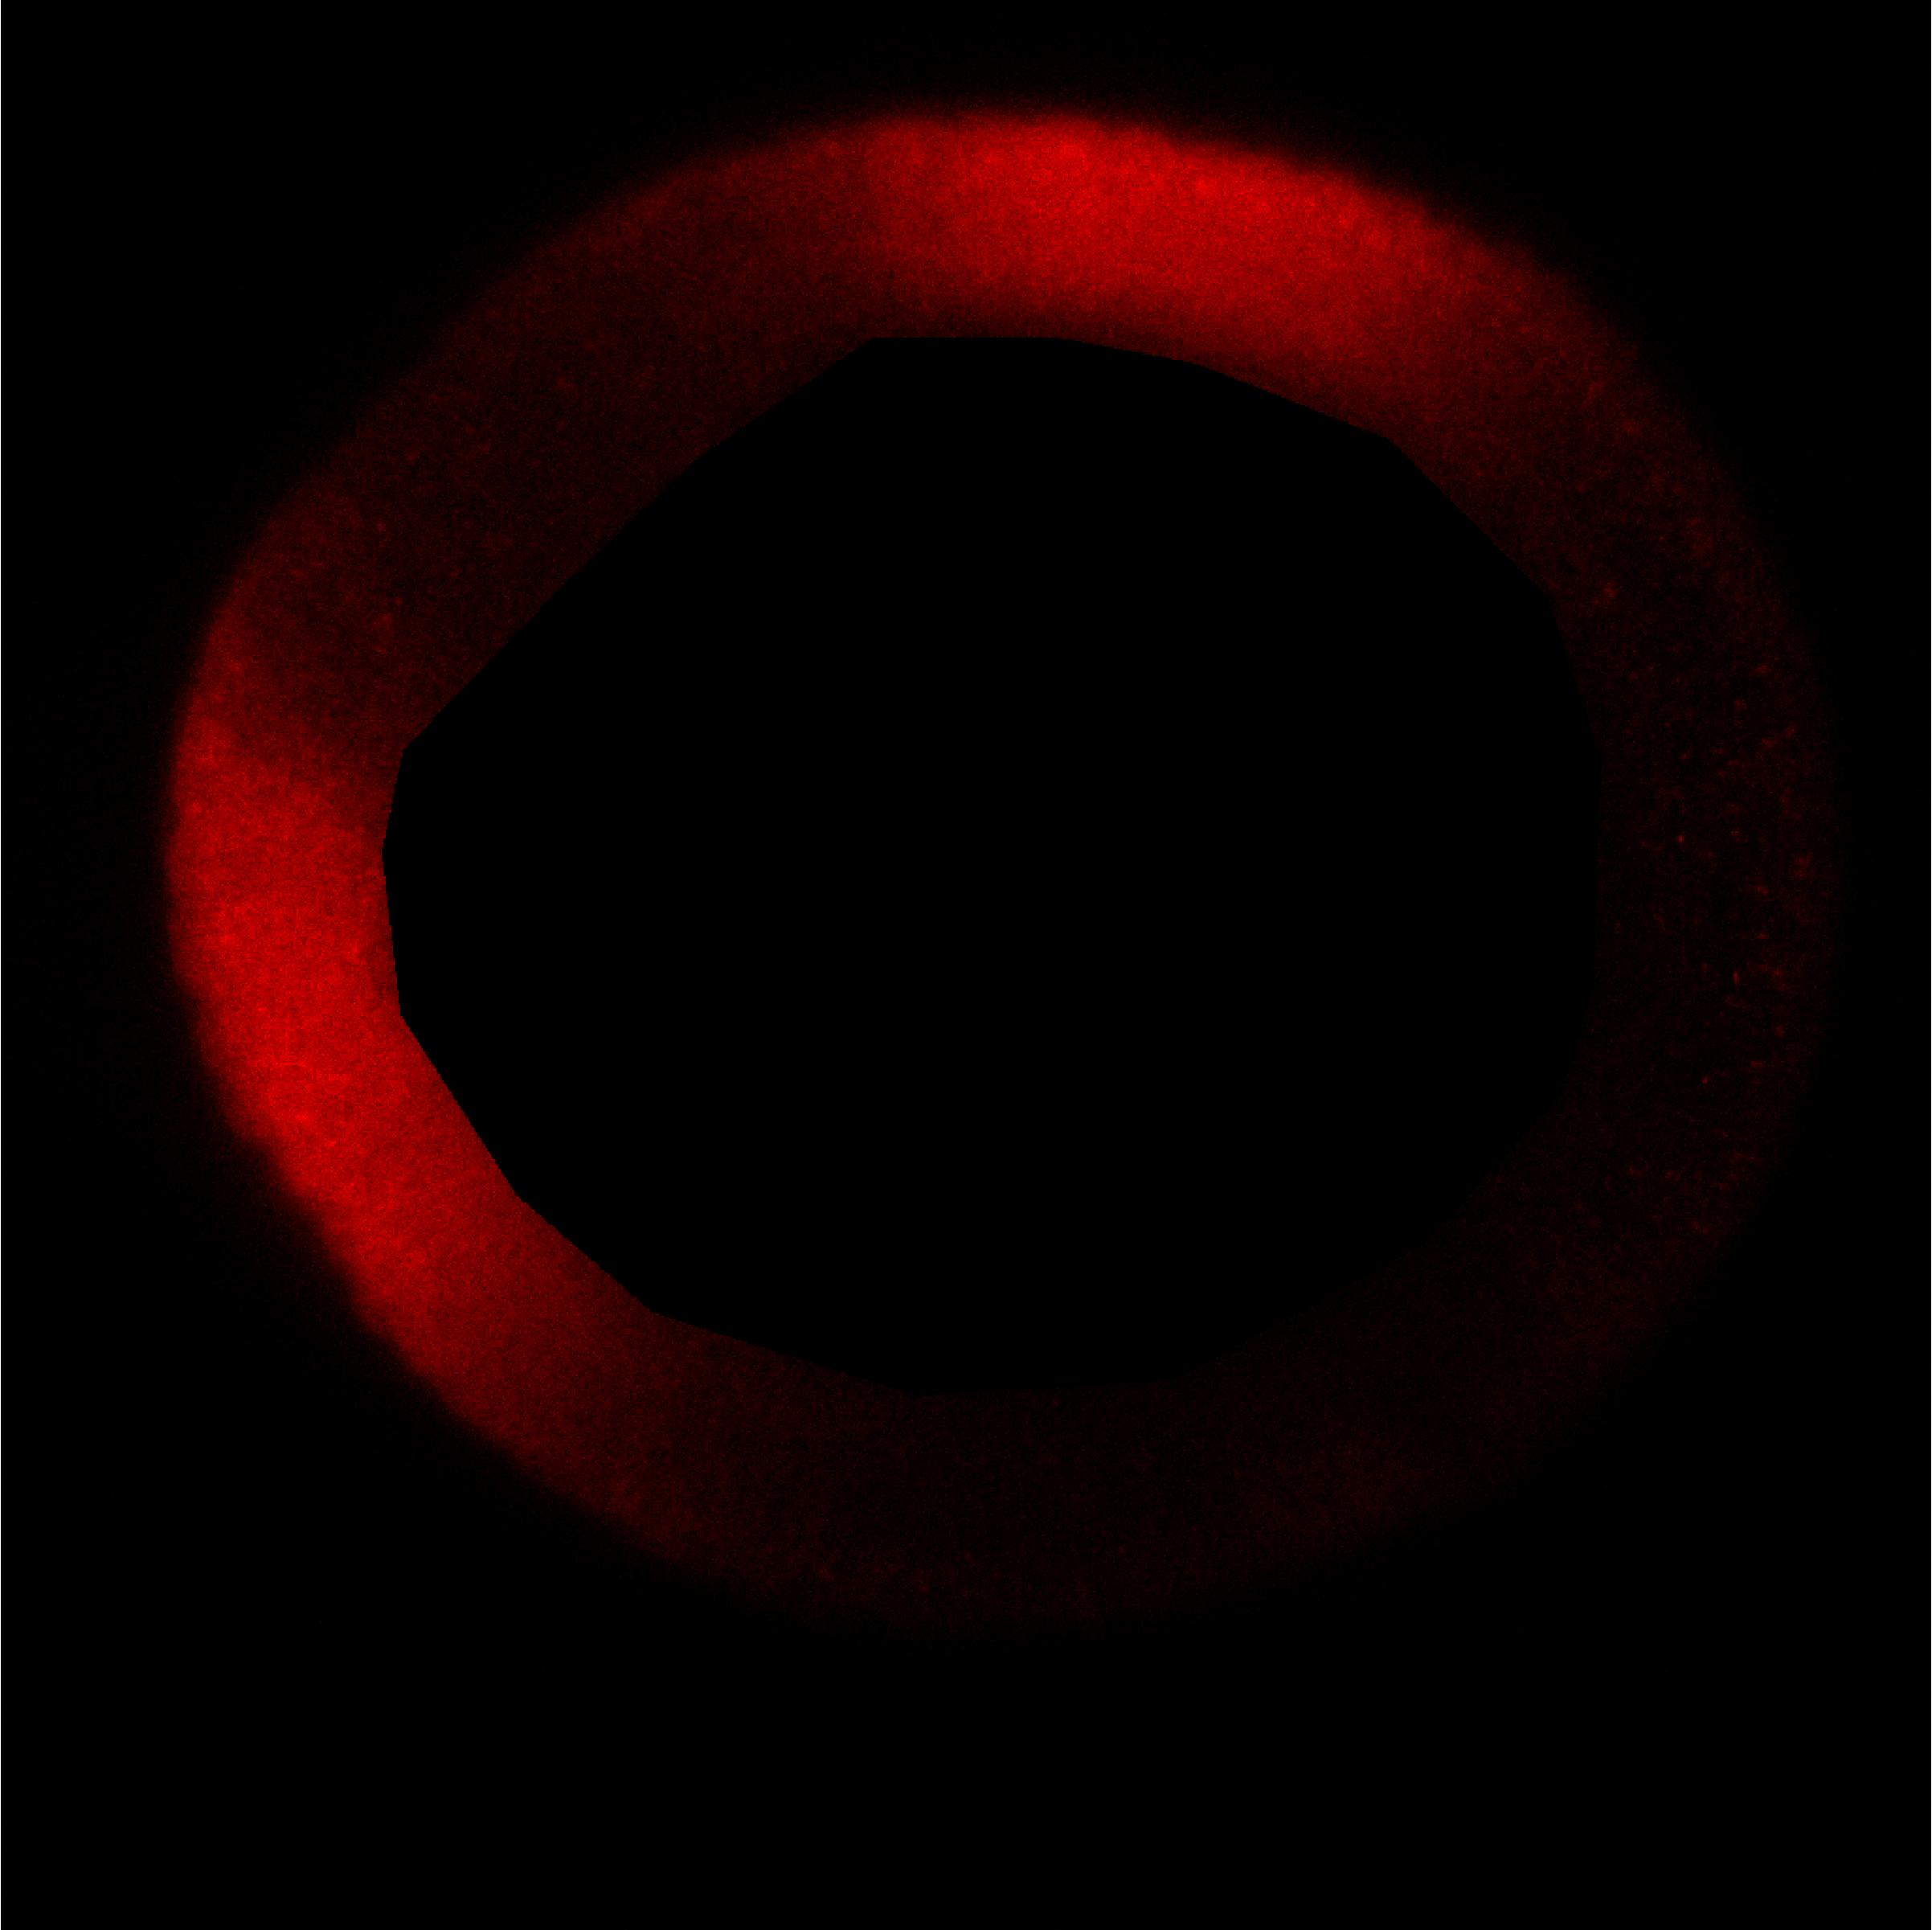
\includegraphics[width=0.3\textwidth]{drosophila_dpERK}};
        		\draw[gray,<->] (dpERKimage.south west) --  (dpERKimage.south east) node[below,midway] { \tiny $100 \mu m$};

        \node[right=of dpERKimage] (dpERKprofile) {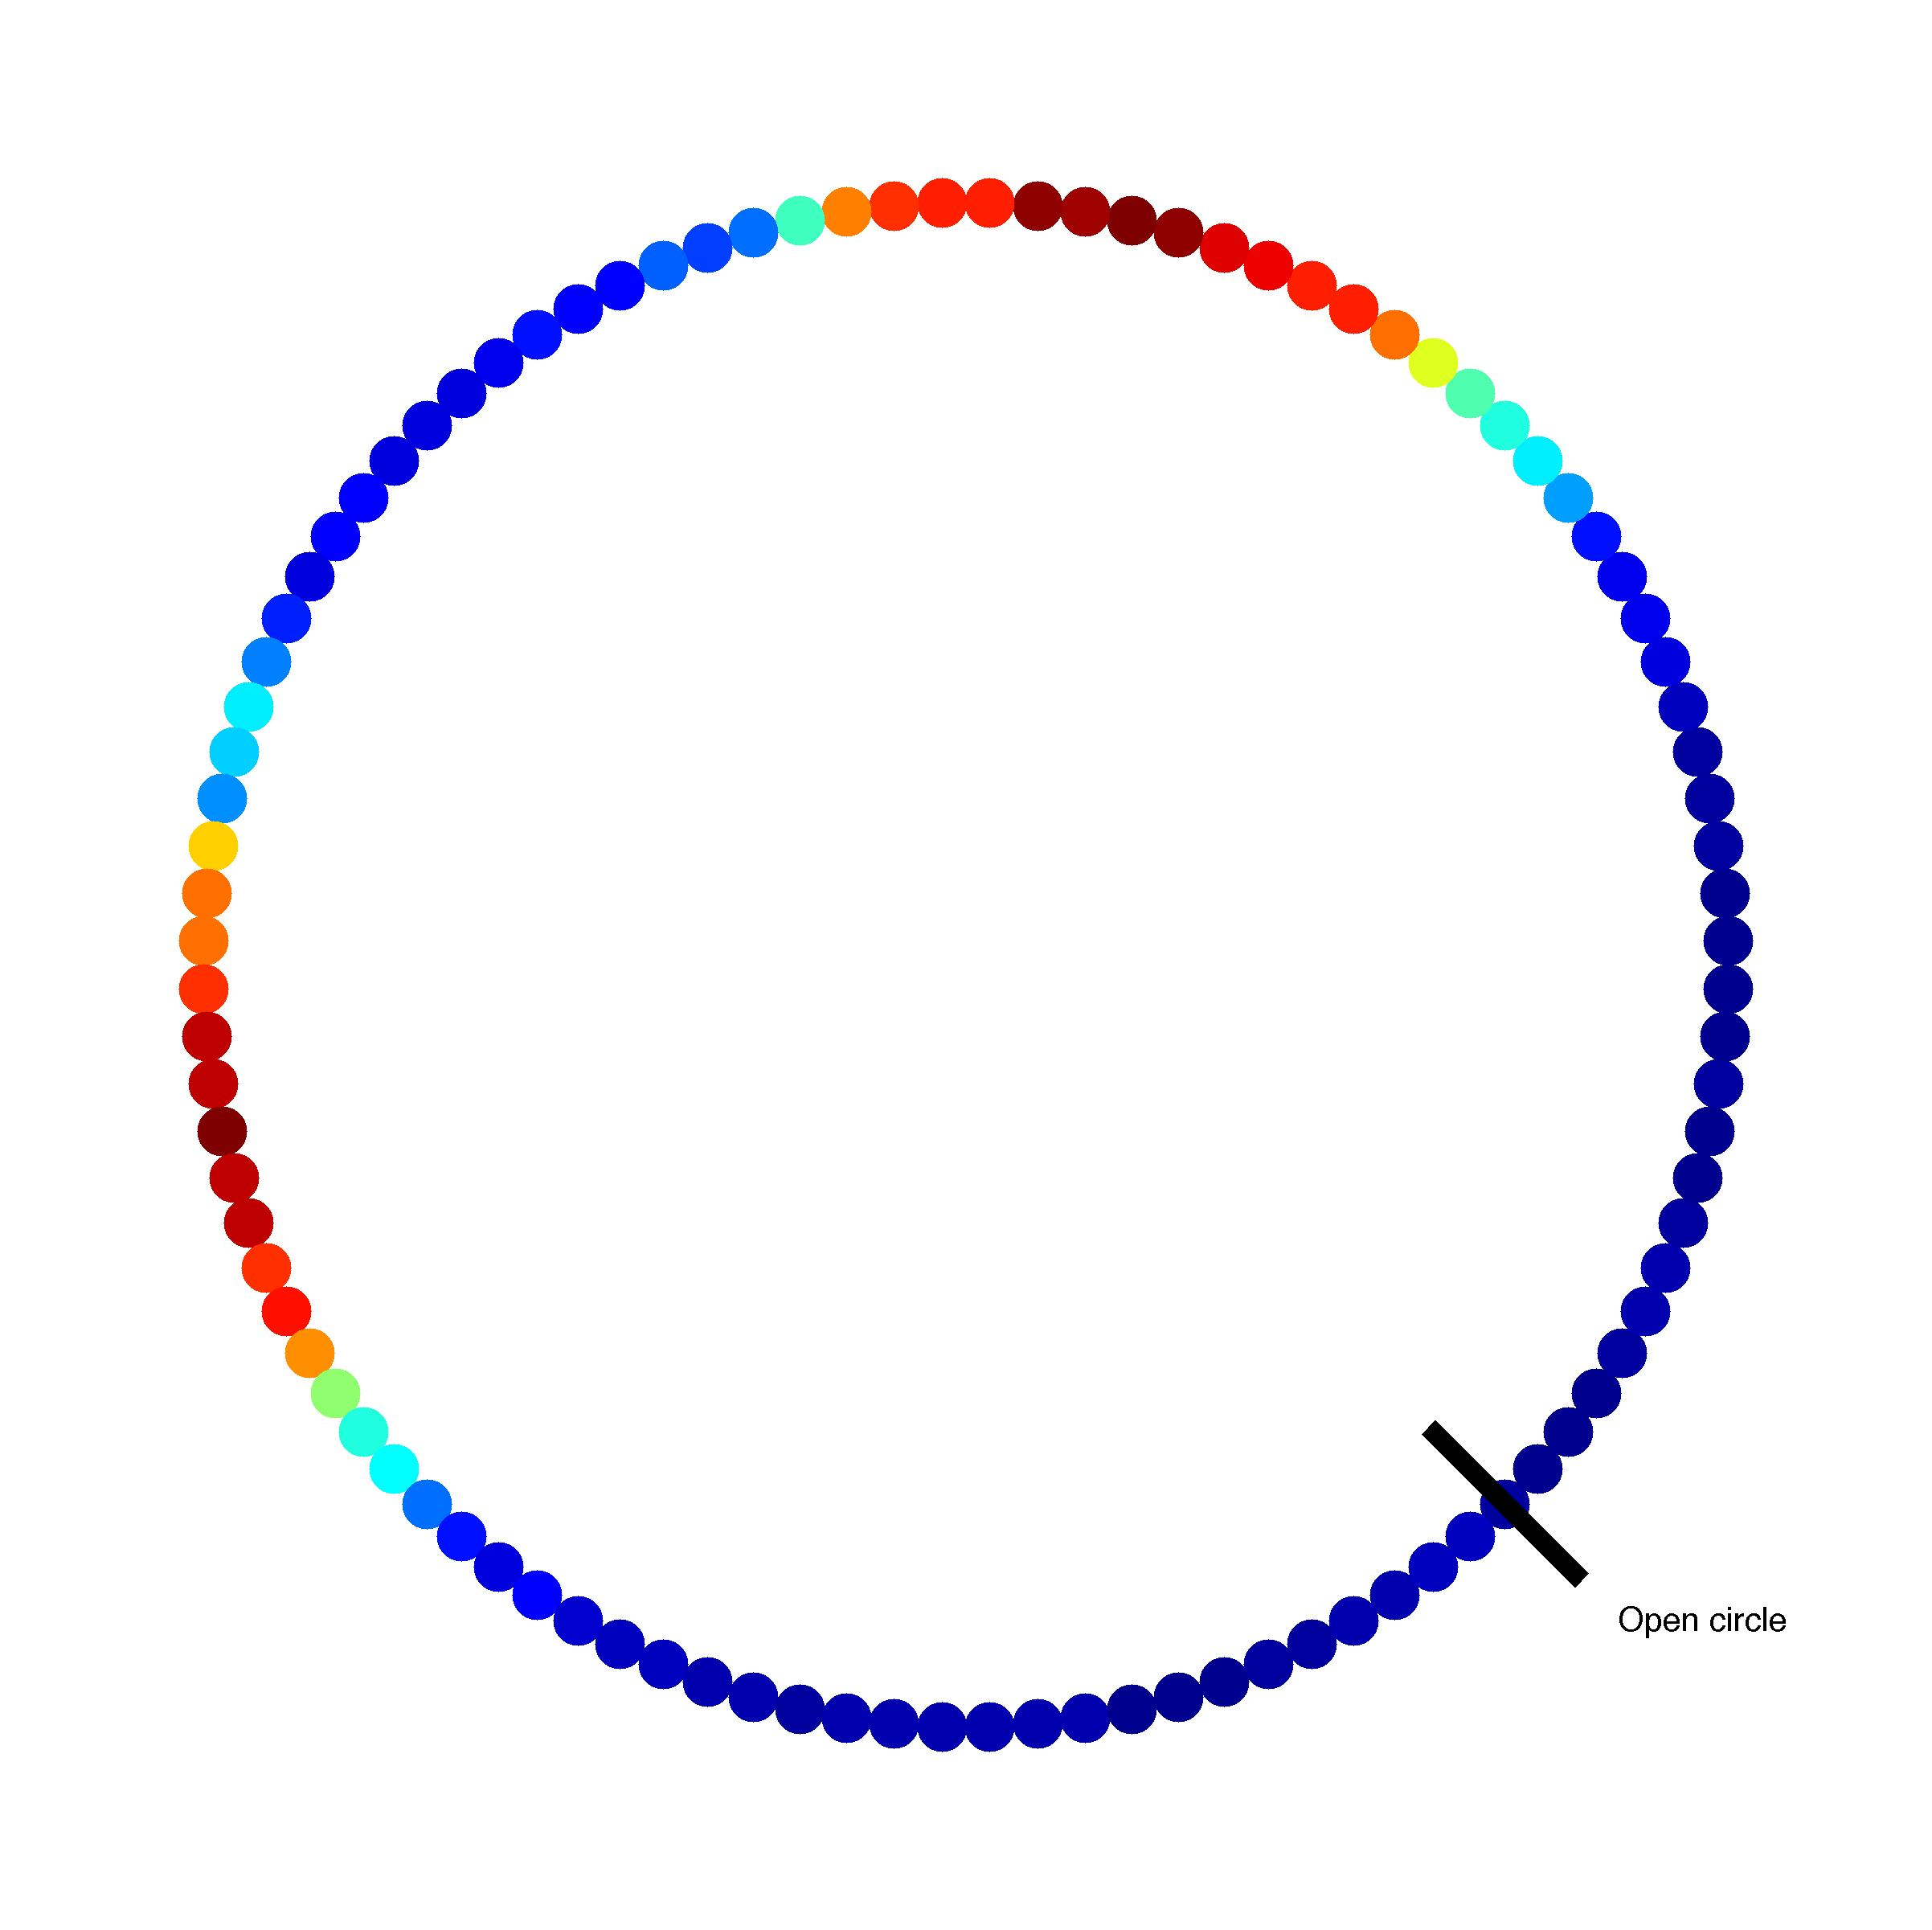
\includegraphics[width=0.3\textwidth]{circle_profile}};
        \draw[->] (dpERKimage)--(dpERKprofile);
    \end{tikzpicture}
    
    However, we could do the same analysis with {\bf raw images} instead of the concentration profiles to extract the dynamics
    
    We must now synchronize/align the images under all {\bf translations and rotations}
    
	\end{frame}

\begin{frame}{Alignment of Two-Dimensional Images}
    We first align and order the images using vector diffusion maps\\
    
    \centering
    \begin{tikzpicture}
    	\node[anchor=south west] (image) {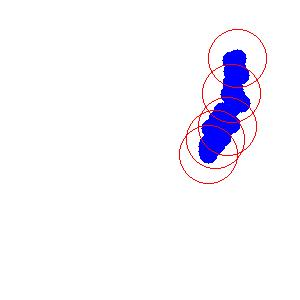
\includegraphics[width=0.5\textwidth]{vdm_2d_time_corr2}};
    	\begin{scope}[x={(image.south east)},y={(image.north west)}]
    	%\draw[help lines,xstep=.05,ystep=.05] (0,0) grid (1,1);
    	\node(x1) at (0.23,0.18) {};
    	\node(x2) at (0.34,0.27) {};
    	\node(x3) at (0.52,0.37) {};
    	\node(x4) at (0.58,0.58) {};
    	\node(x5) at (0.67,0.81) {};
    	\end{scope}
    	\node[below=0.2in of image](fig3) {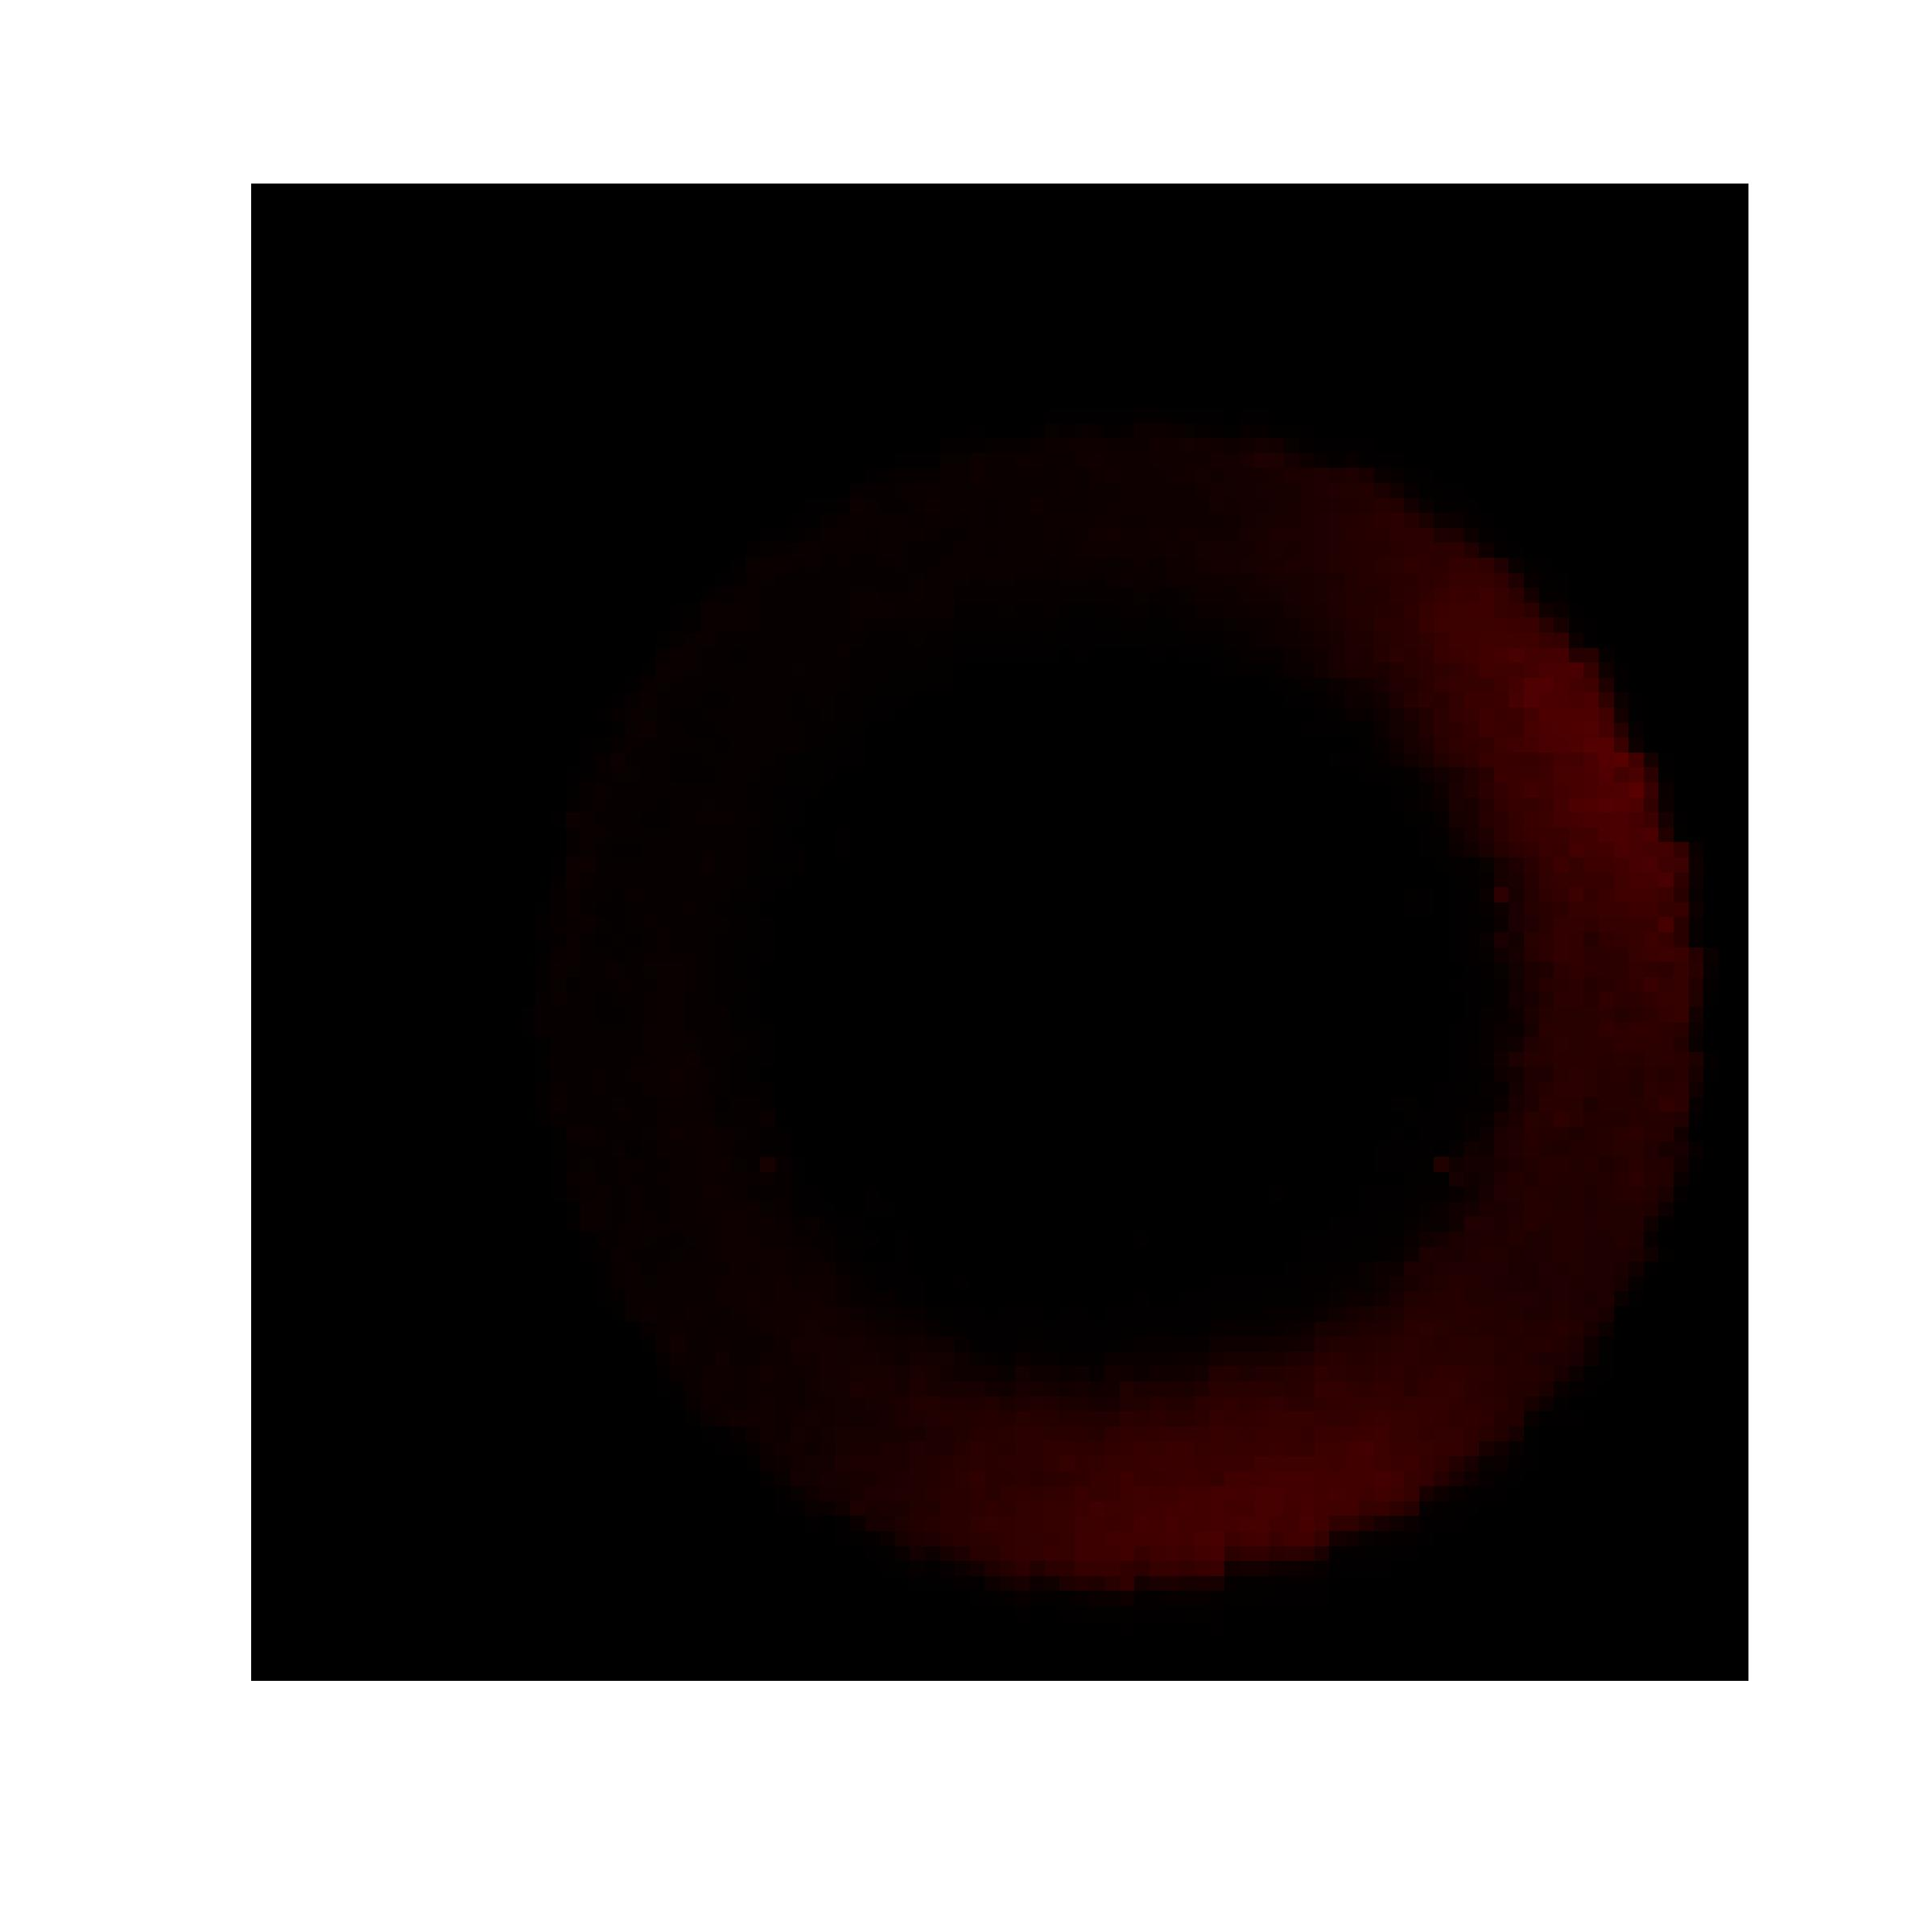
\includegraphics[width=0.15\textwidth]{dpERK_vdm_3}};		
    	\node[left=0.1in of fig3](fig2) {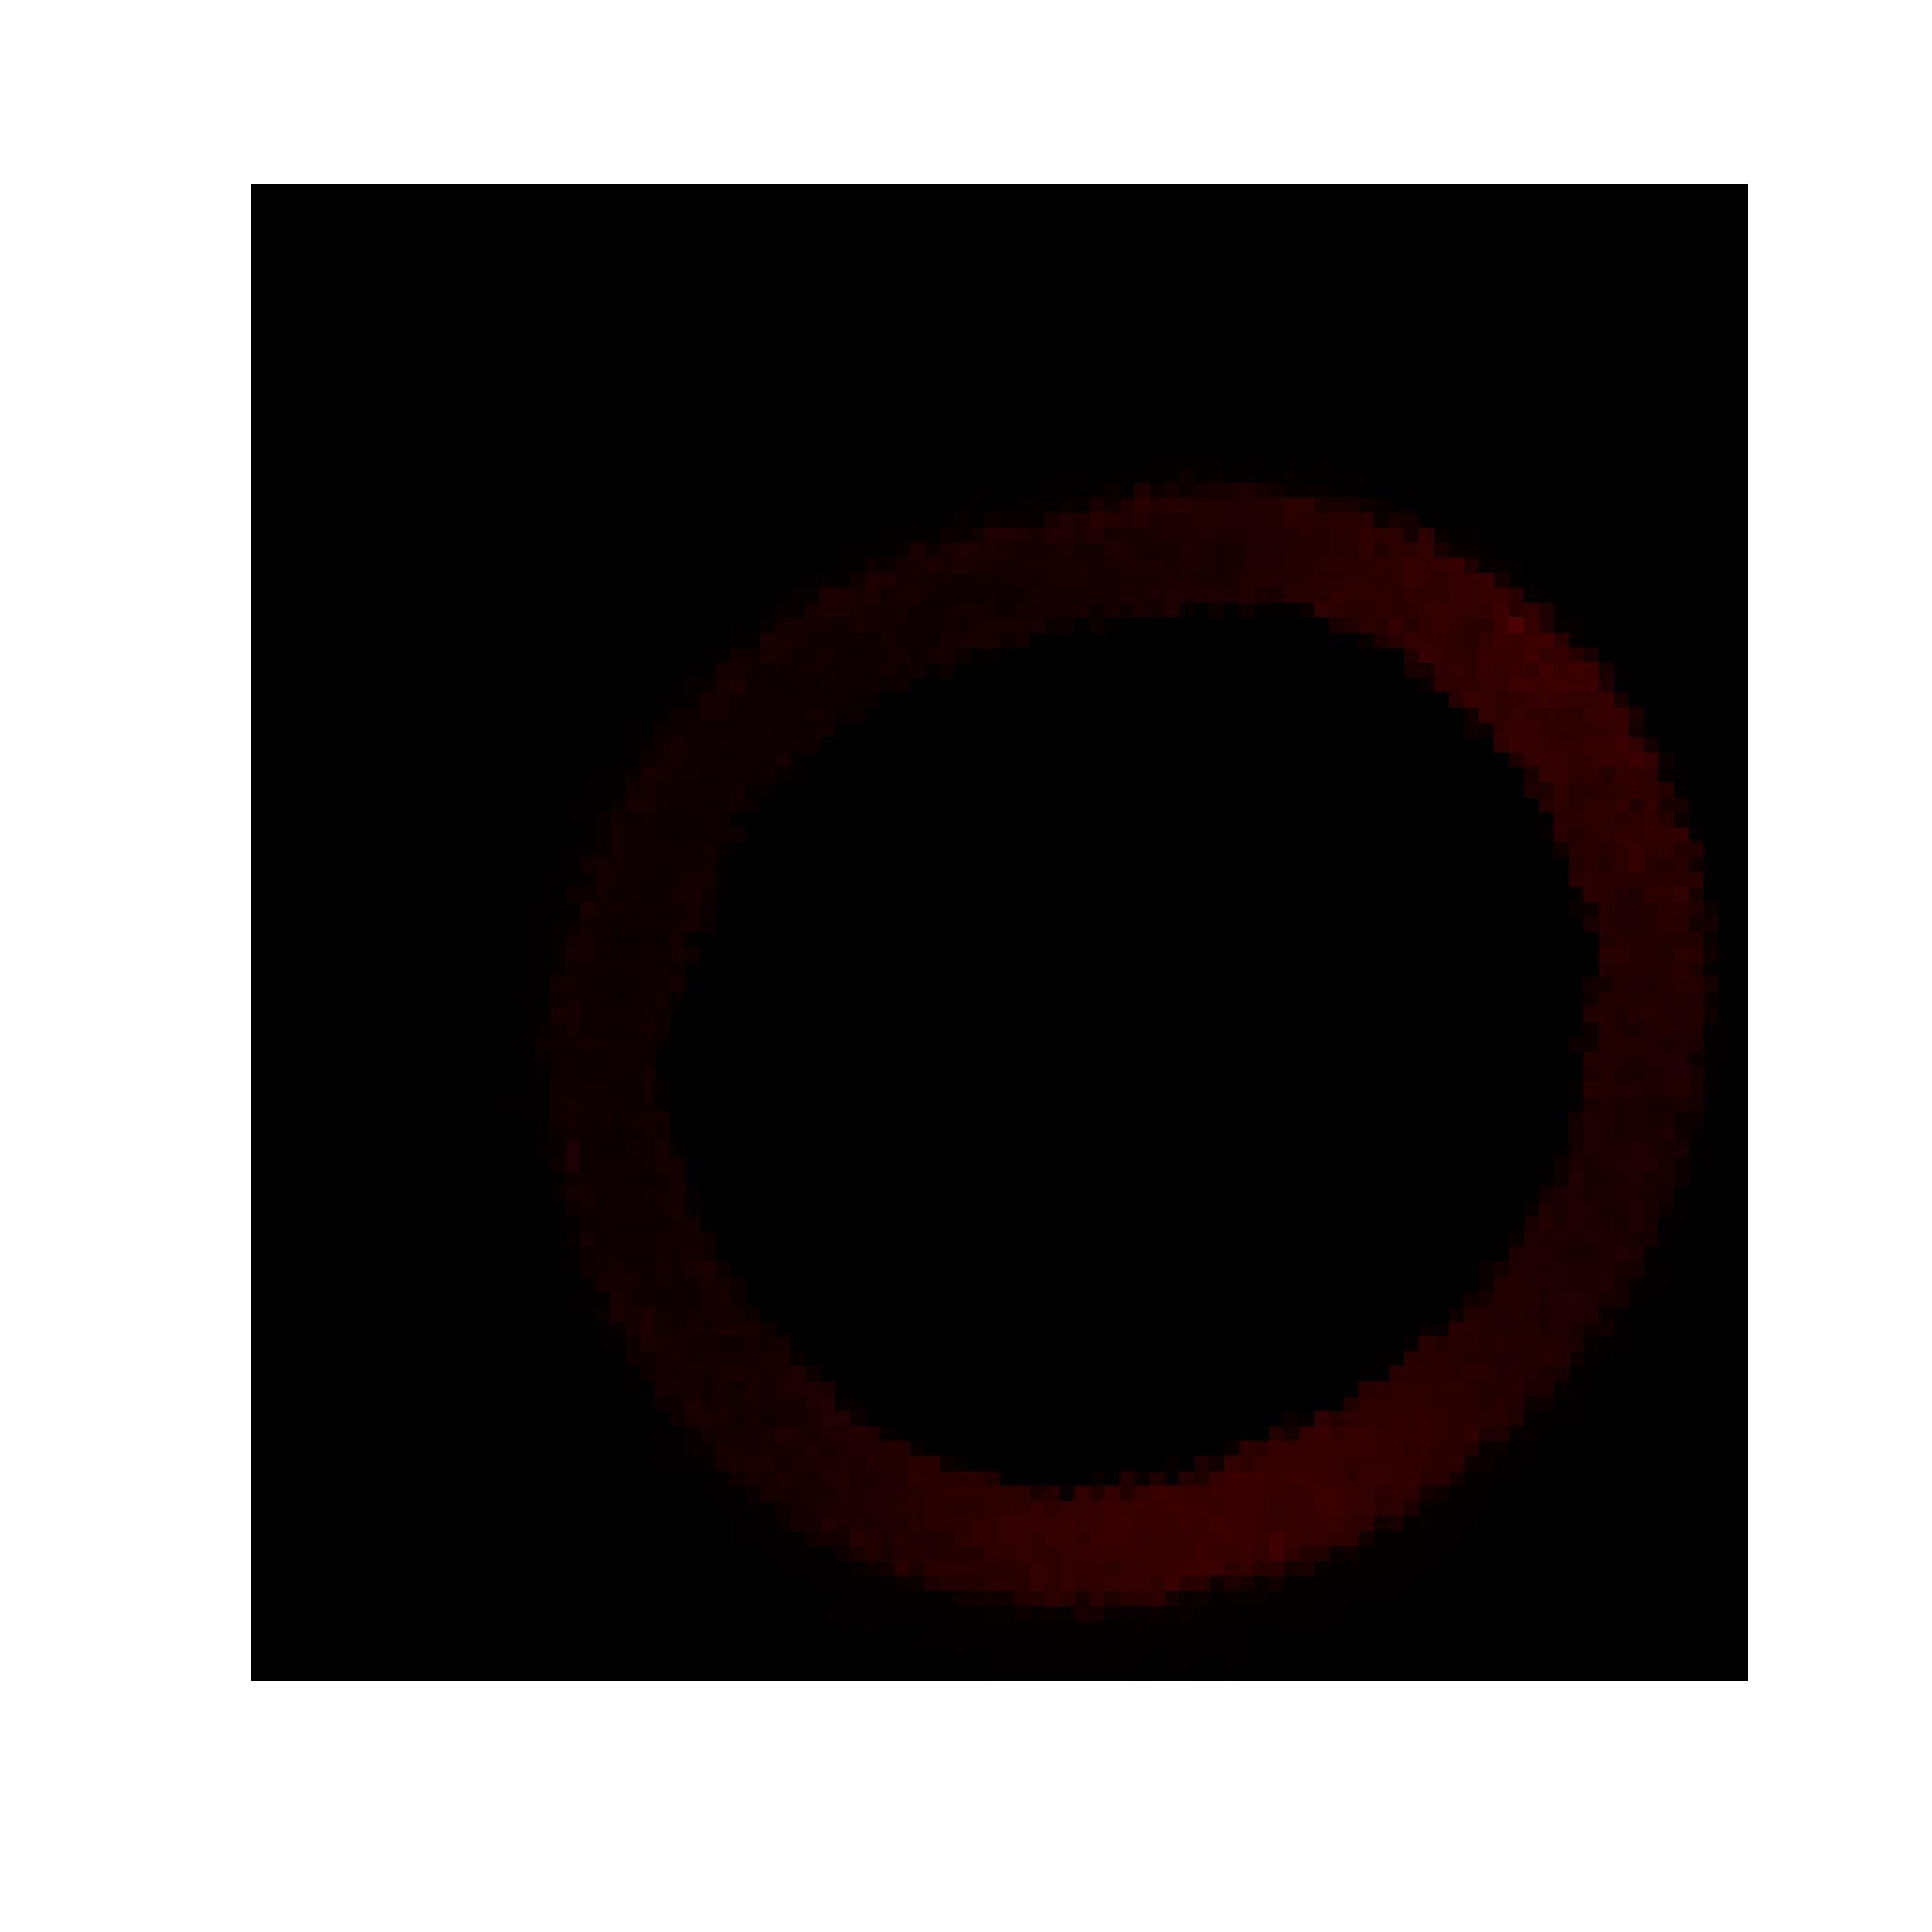
\includegraphics[width=0.15\textwidth]{dpERK_vdm_2}};
    	\node[left=0.1in of fig2](fig1) {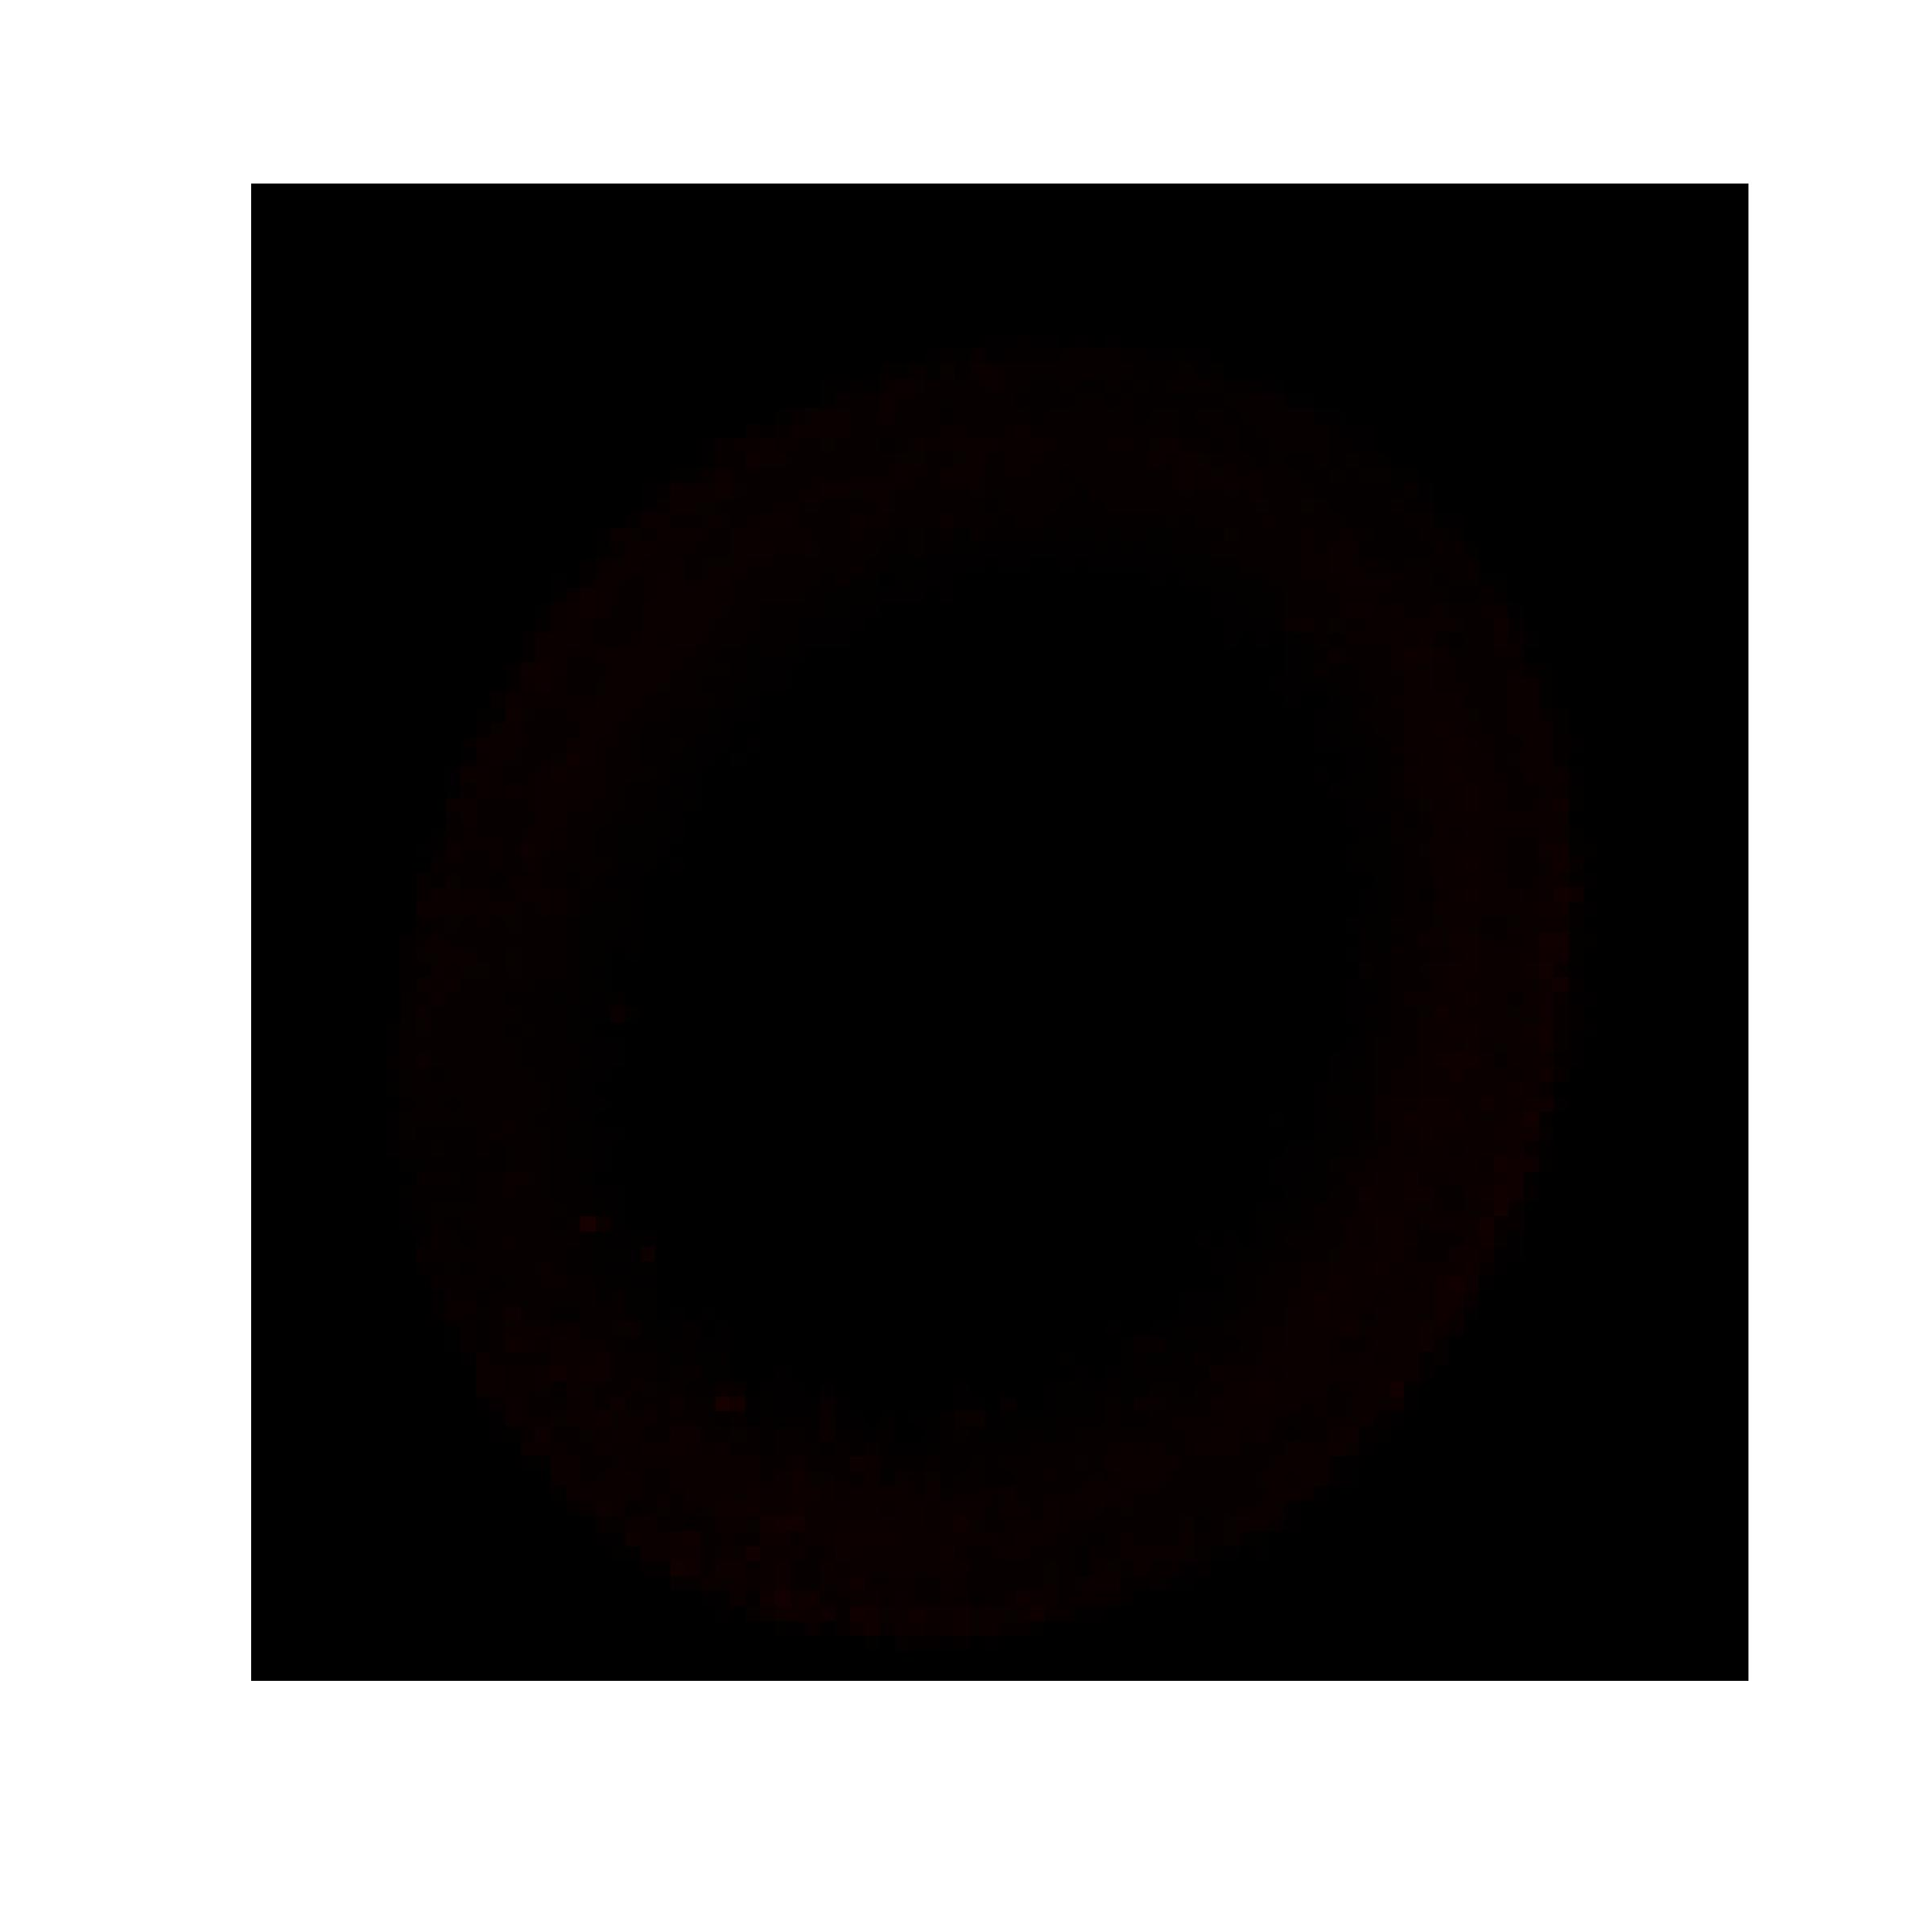
\includegraphics[width=0.15\textwidth]{dpERK_vdm_1}};	
    	\node[right=0.1in of fig3](fig4) {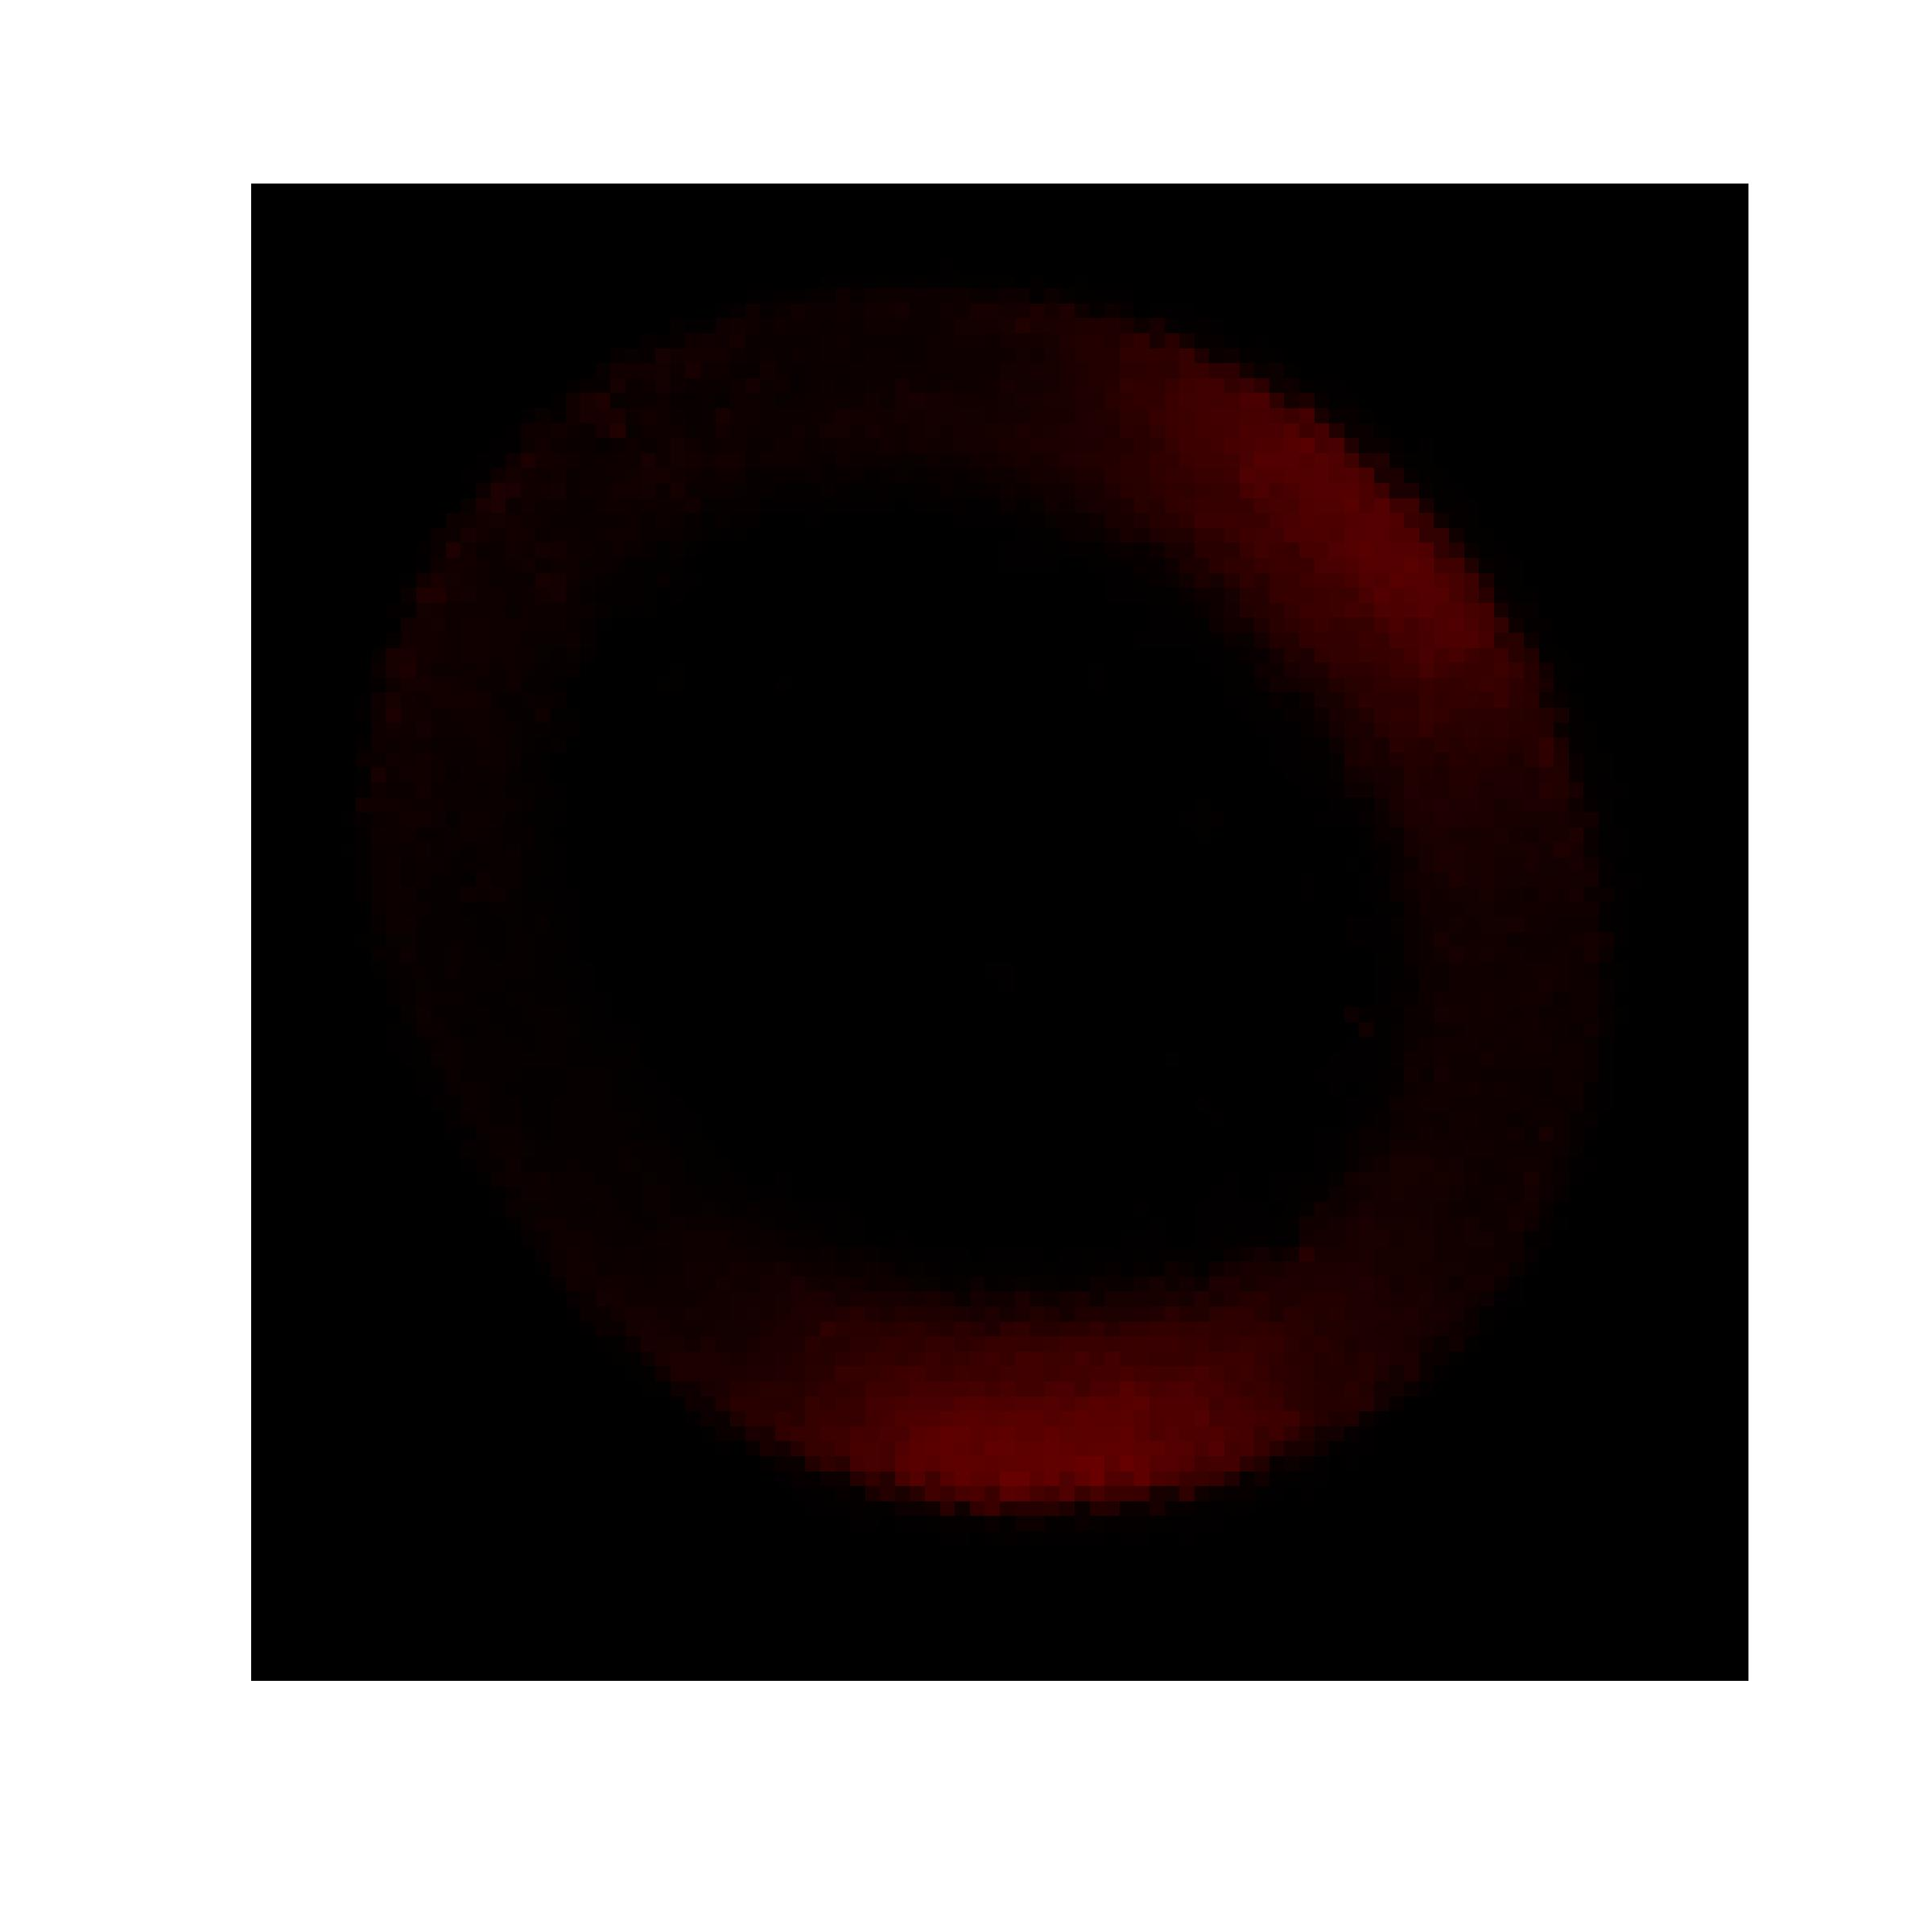
\includegraphics[width=0.15\textwidth]{dpERK_vdm_4}};					
    	\node[right=0.1in of fig4](fig5) {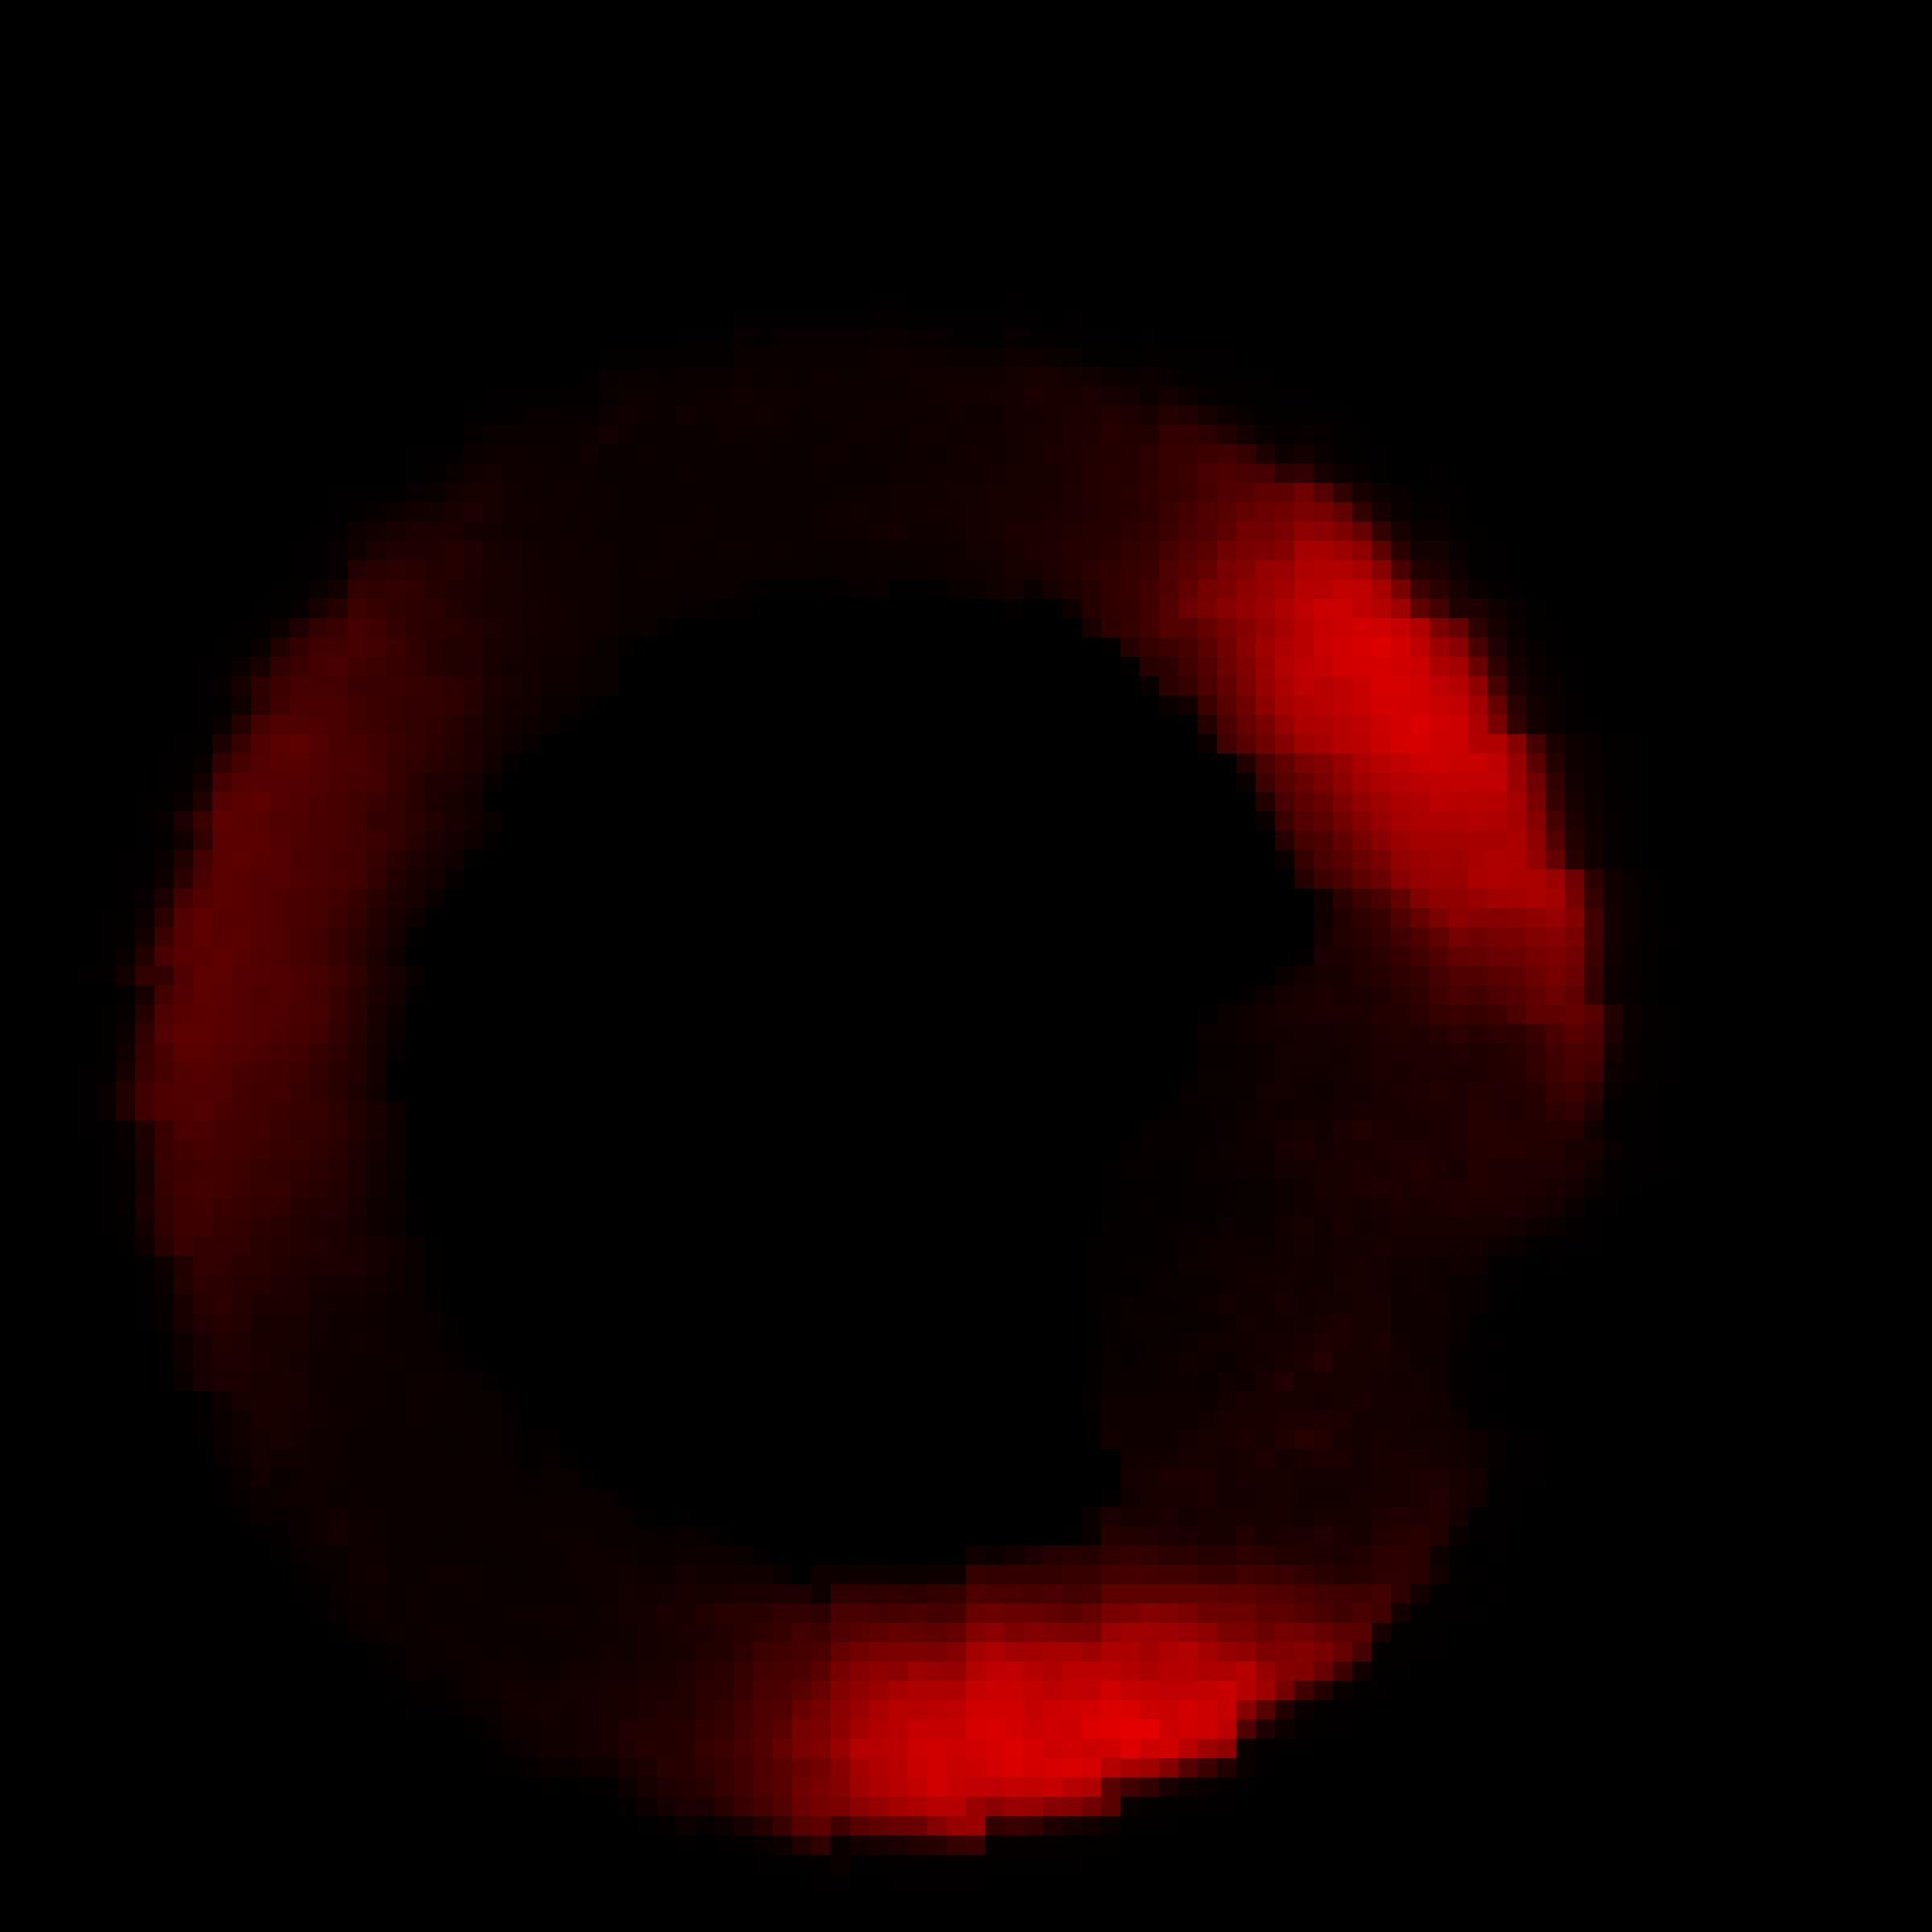
\includegraphics[width=0.15\textwidth]{dpERK_vdm_5}};	    
    	\draw[->] (x1) -- (fig1.north);
    	\draw[->] (x2) -- (fig2.north);
    	\draw[->] (x3) -- (fig3.north);
    	\draw[->] (x4) -- (fig4.north);
    	\draw[->] (x5) -- (fig5.north);
    \end{tikzpicture}
    
\end{frame}

\begin{frame}{Ordering of Two-Dimensional Images}
    We  order the images using the scattering transform + DMAPS\\
    
    \centering
    \begin{tikzpicture}
    	\node[anchor=south west] (image) {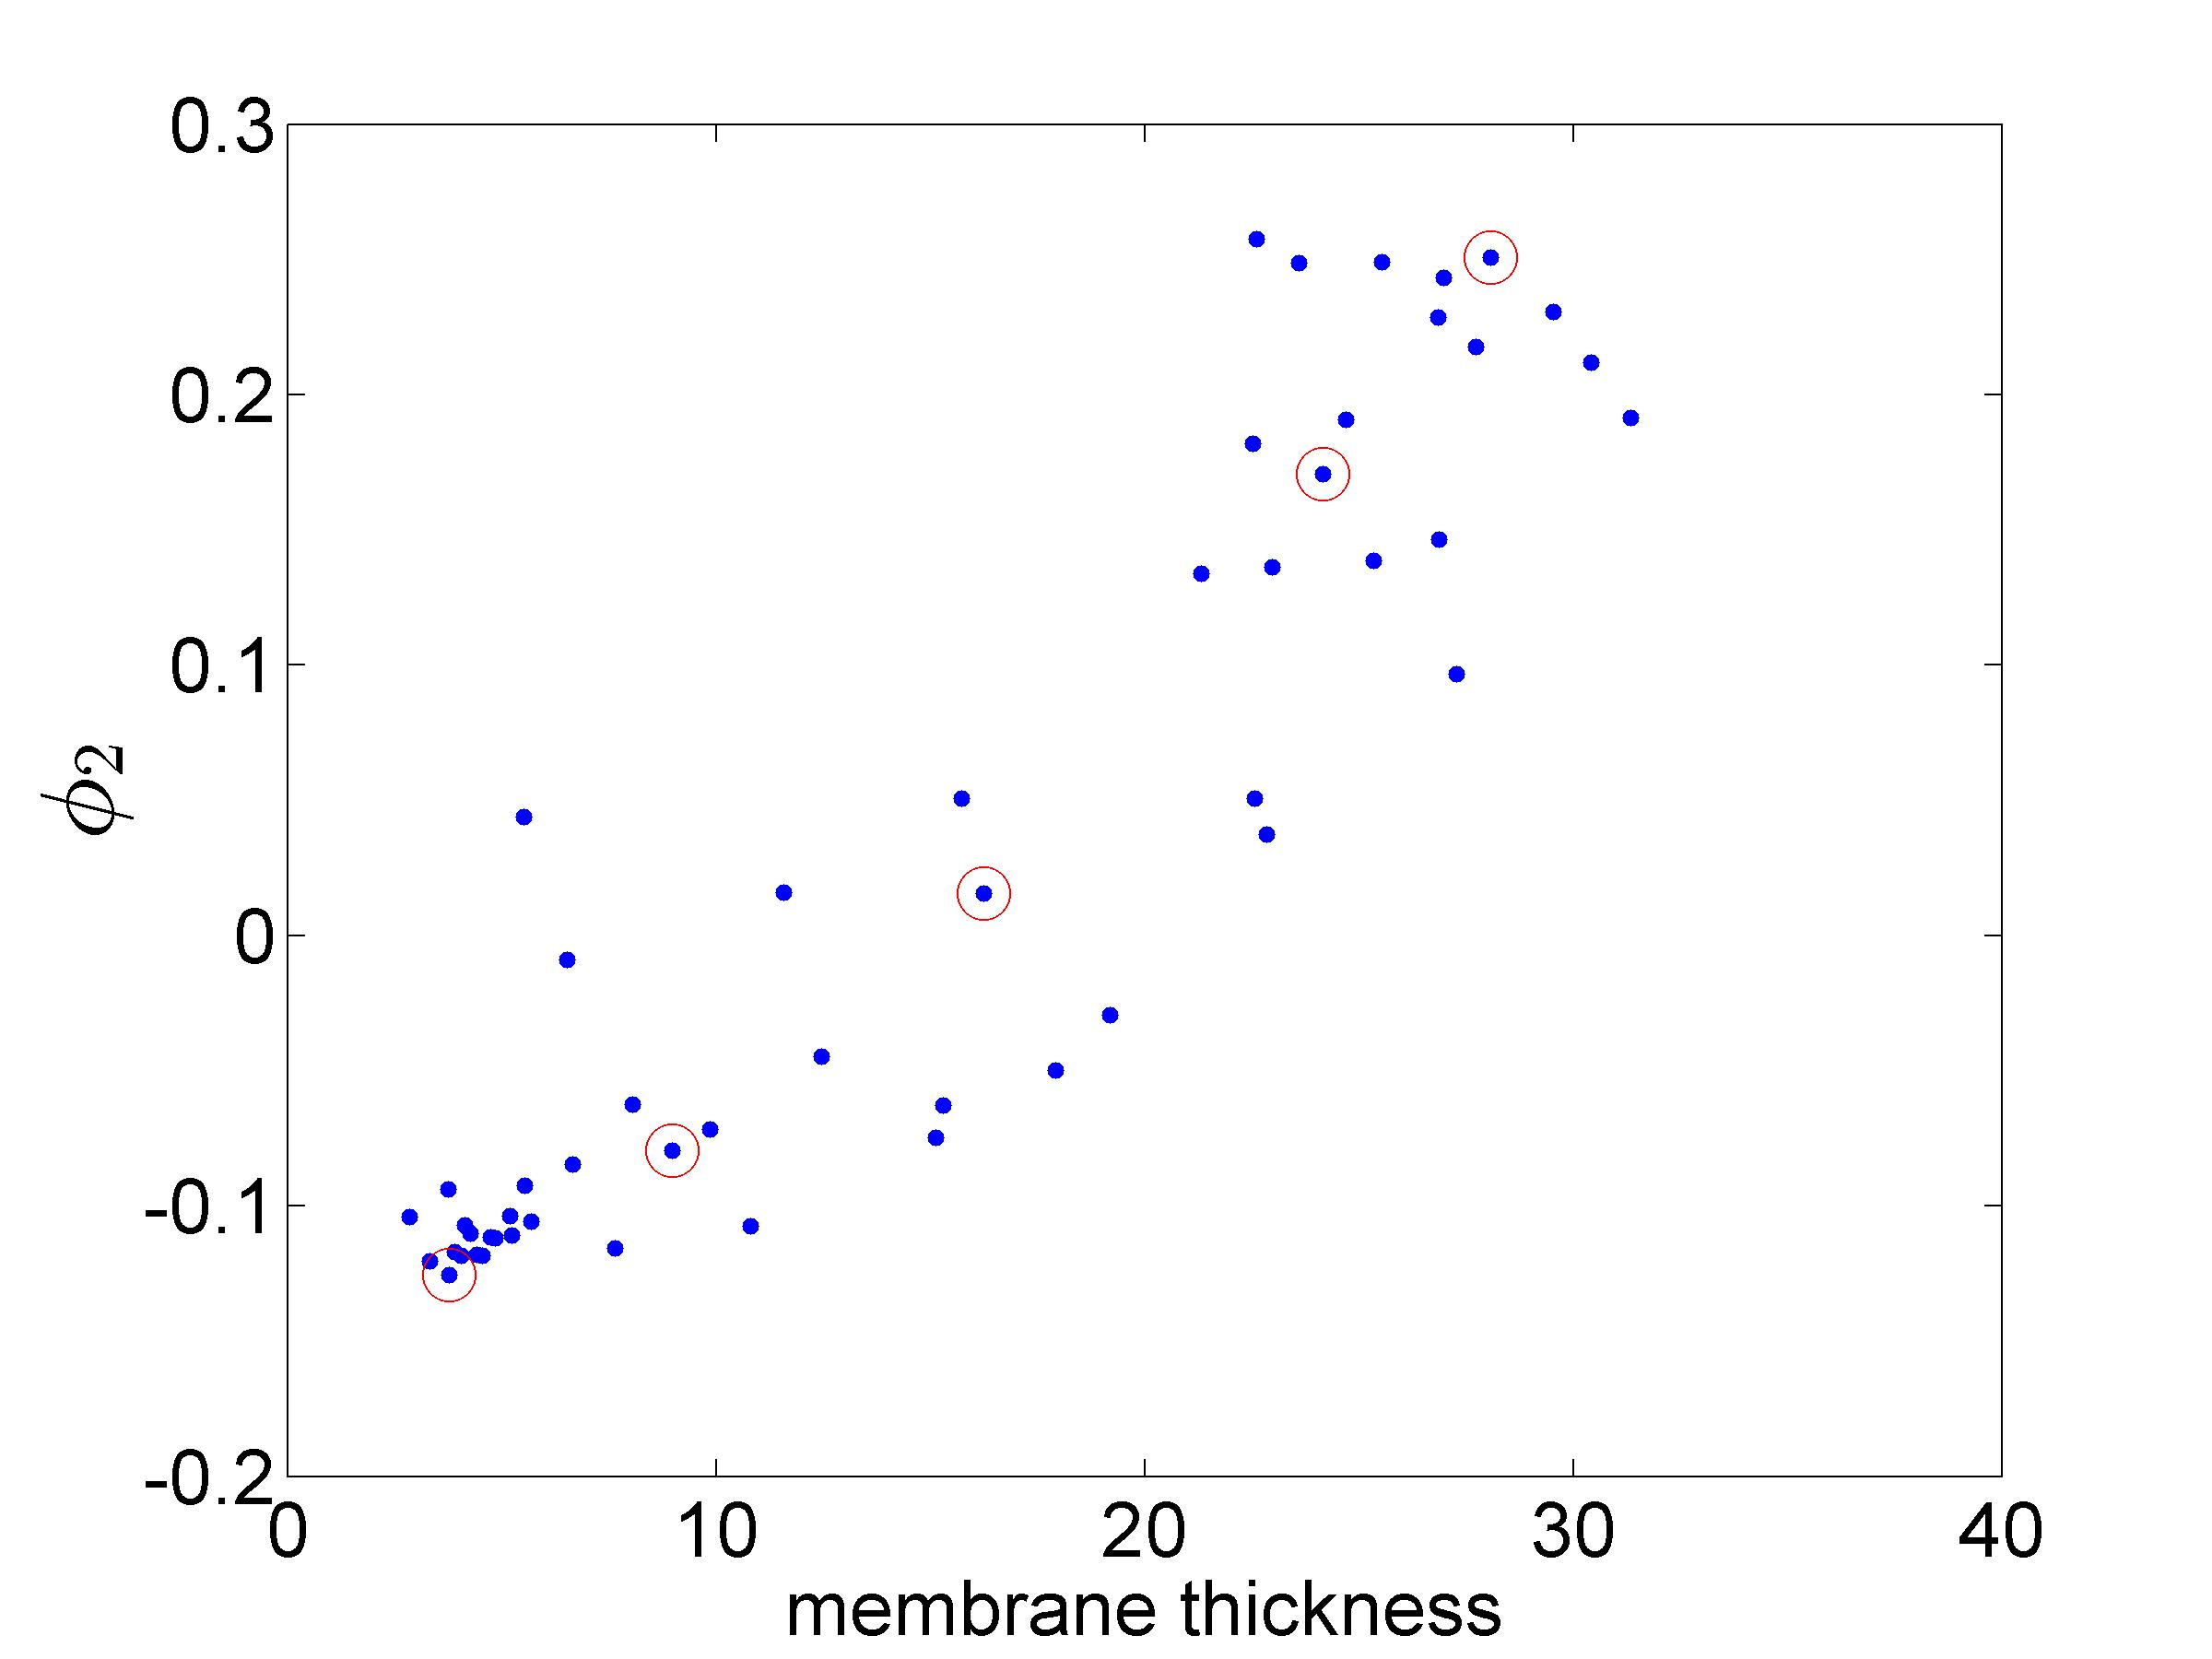
\includegraphics[width=0.5\textwidth]{DMAPS_scat_time_corr2}};
    	\begin{scope}[x={(image.south east)},y={(image.north west)}]
    	%\draw[help lines,xstep=.05,ystep=.05] (0,0) grid (1,1);
    	\node(x1) at (0.23,0.24) {};
    	\node(x2) at (0.32,0.32) {};
    	\node(x3) at (0.45,0.49) {};
    	\node(x4) at (0.59,0.72) {};
    	\node(x5) at (0.66,0.85) {};
    	\end{scope}
    	\node[below=0.2in of image](fig3) {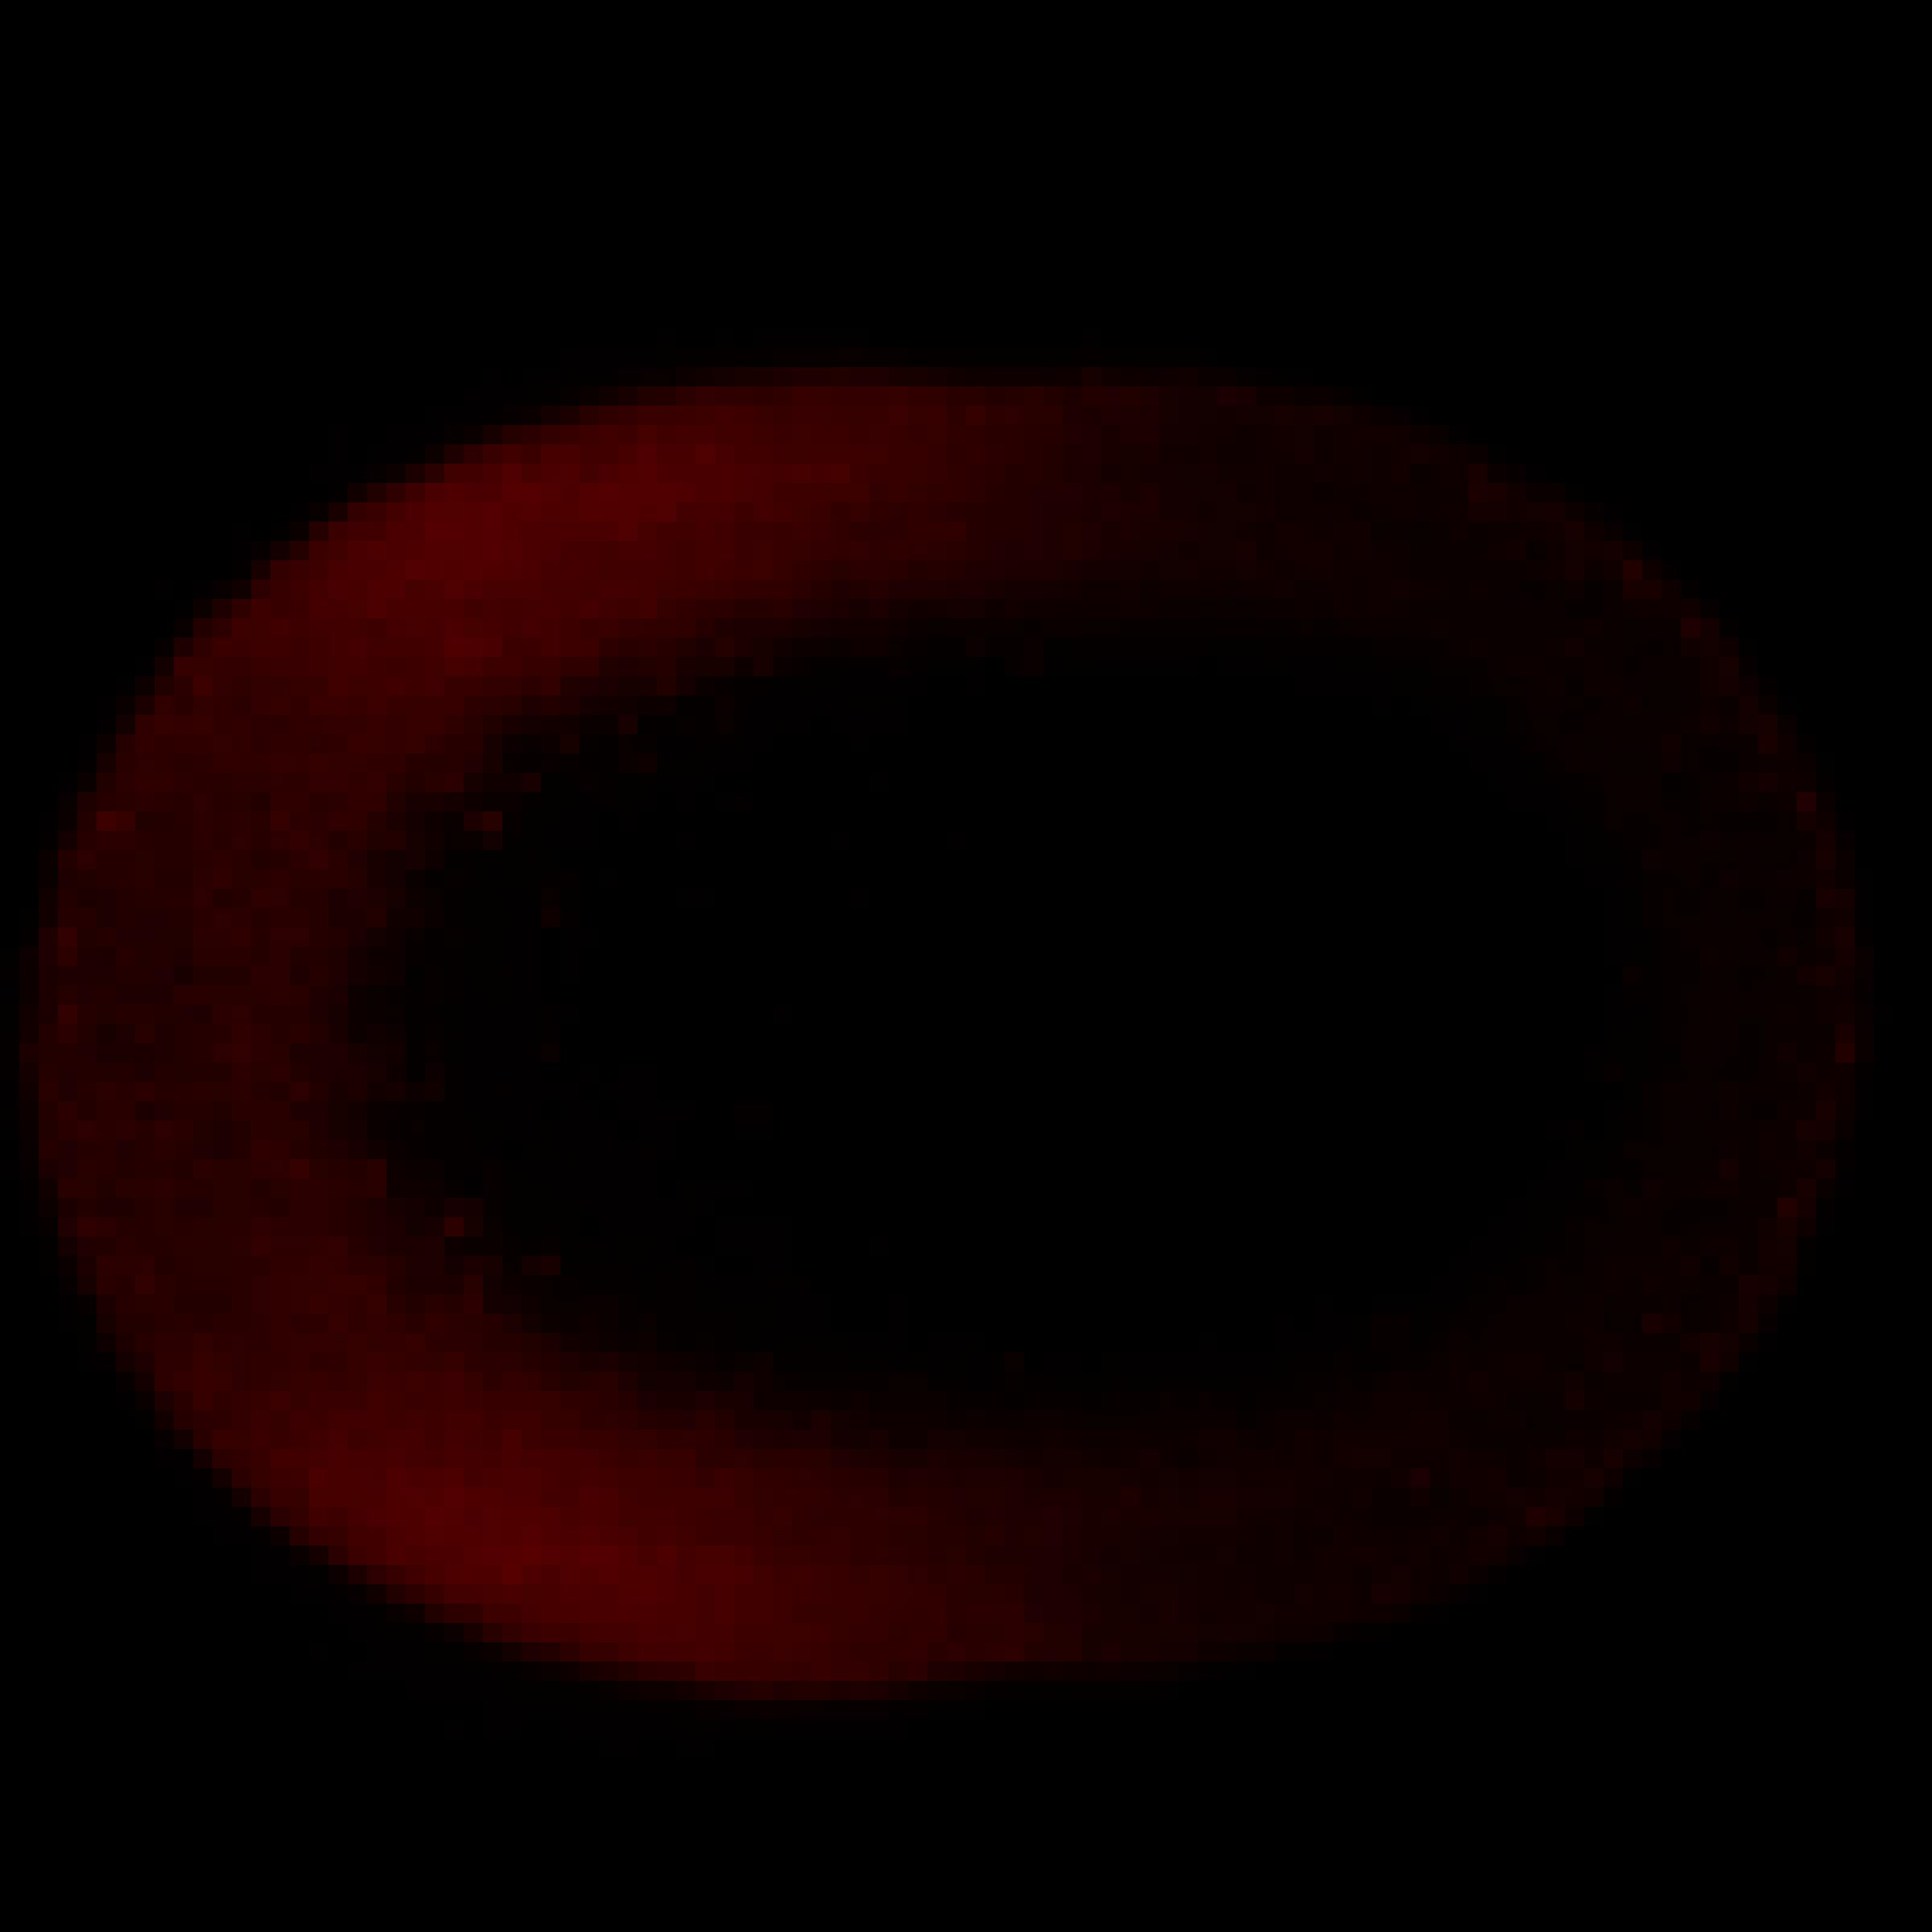
\includegraphics[width=0.15\textwidth]{dpERK_scat_3}};		
    	\node[left=0.1in of fig3](fig2) {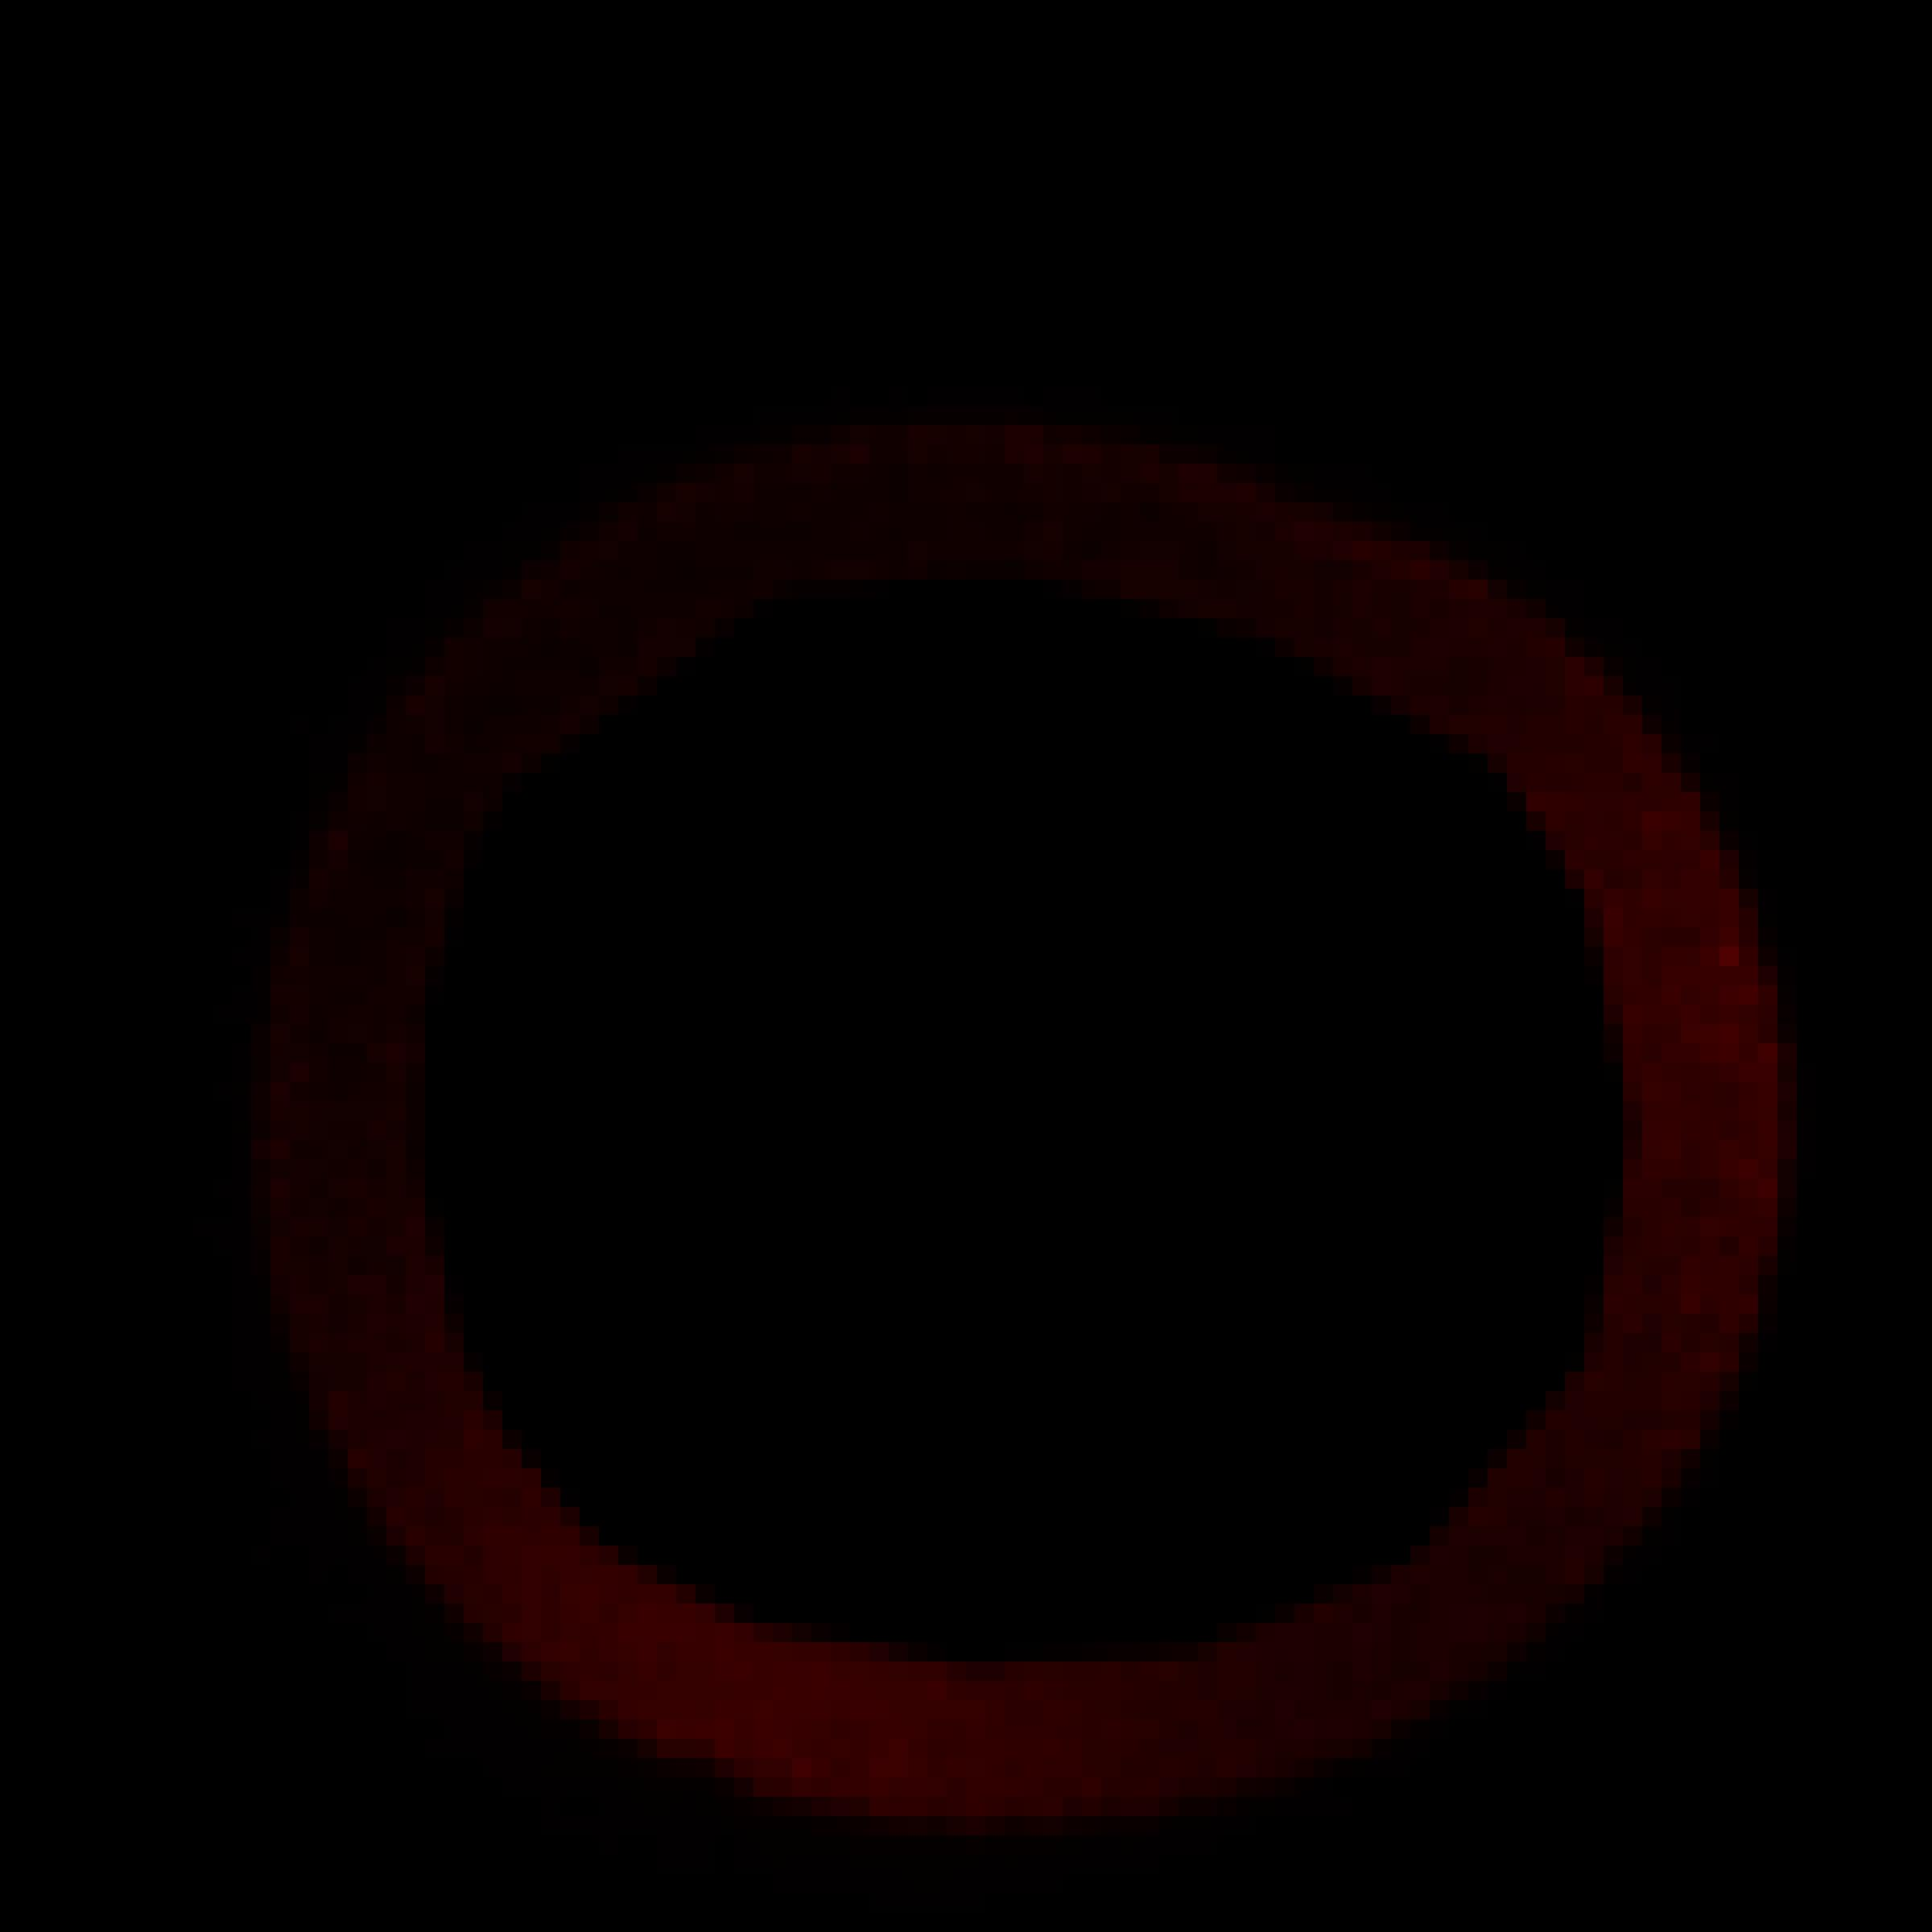
\includegraphics[width=0.15\textwidth]{dpERK_scat_2}};
    	\node[left=0.1in of fig2](fig1) {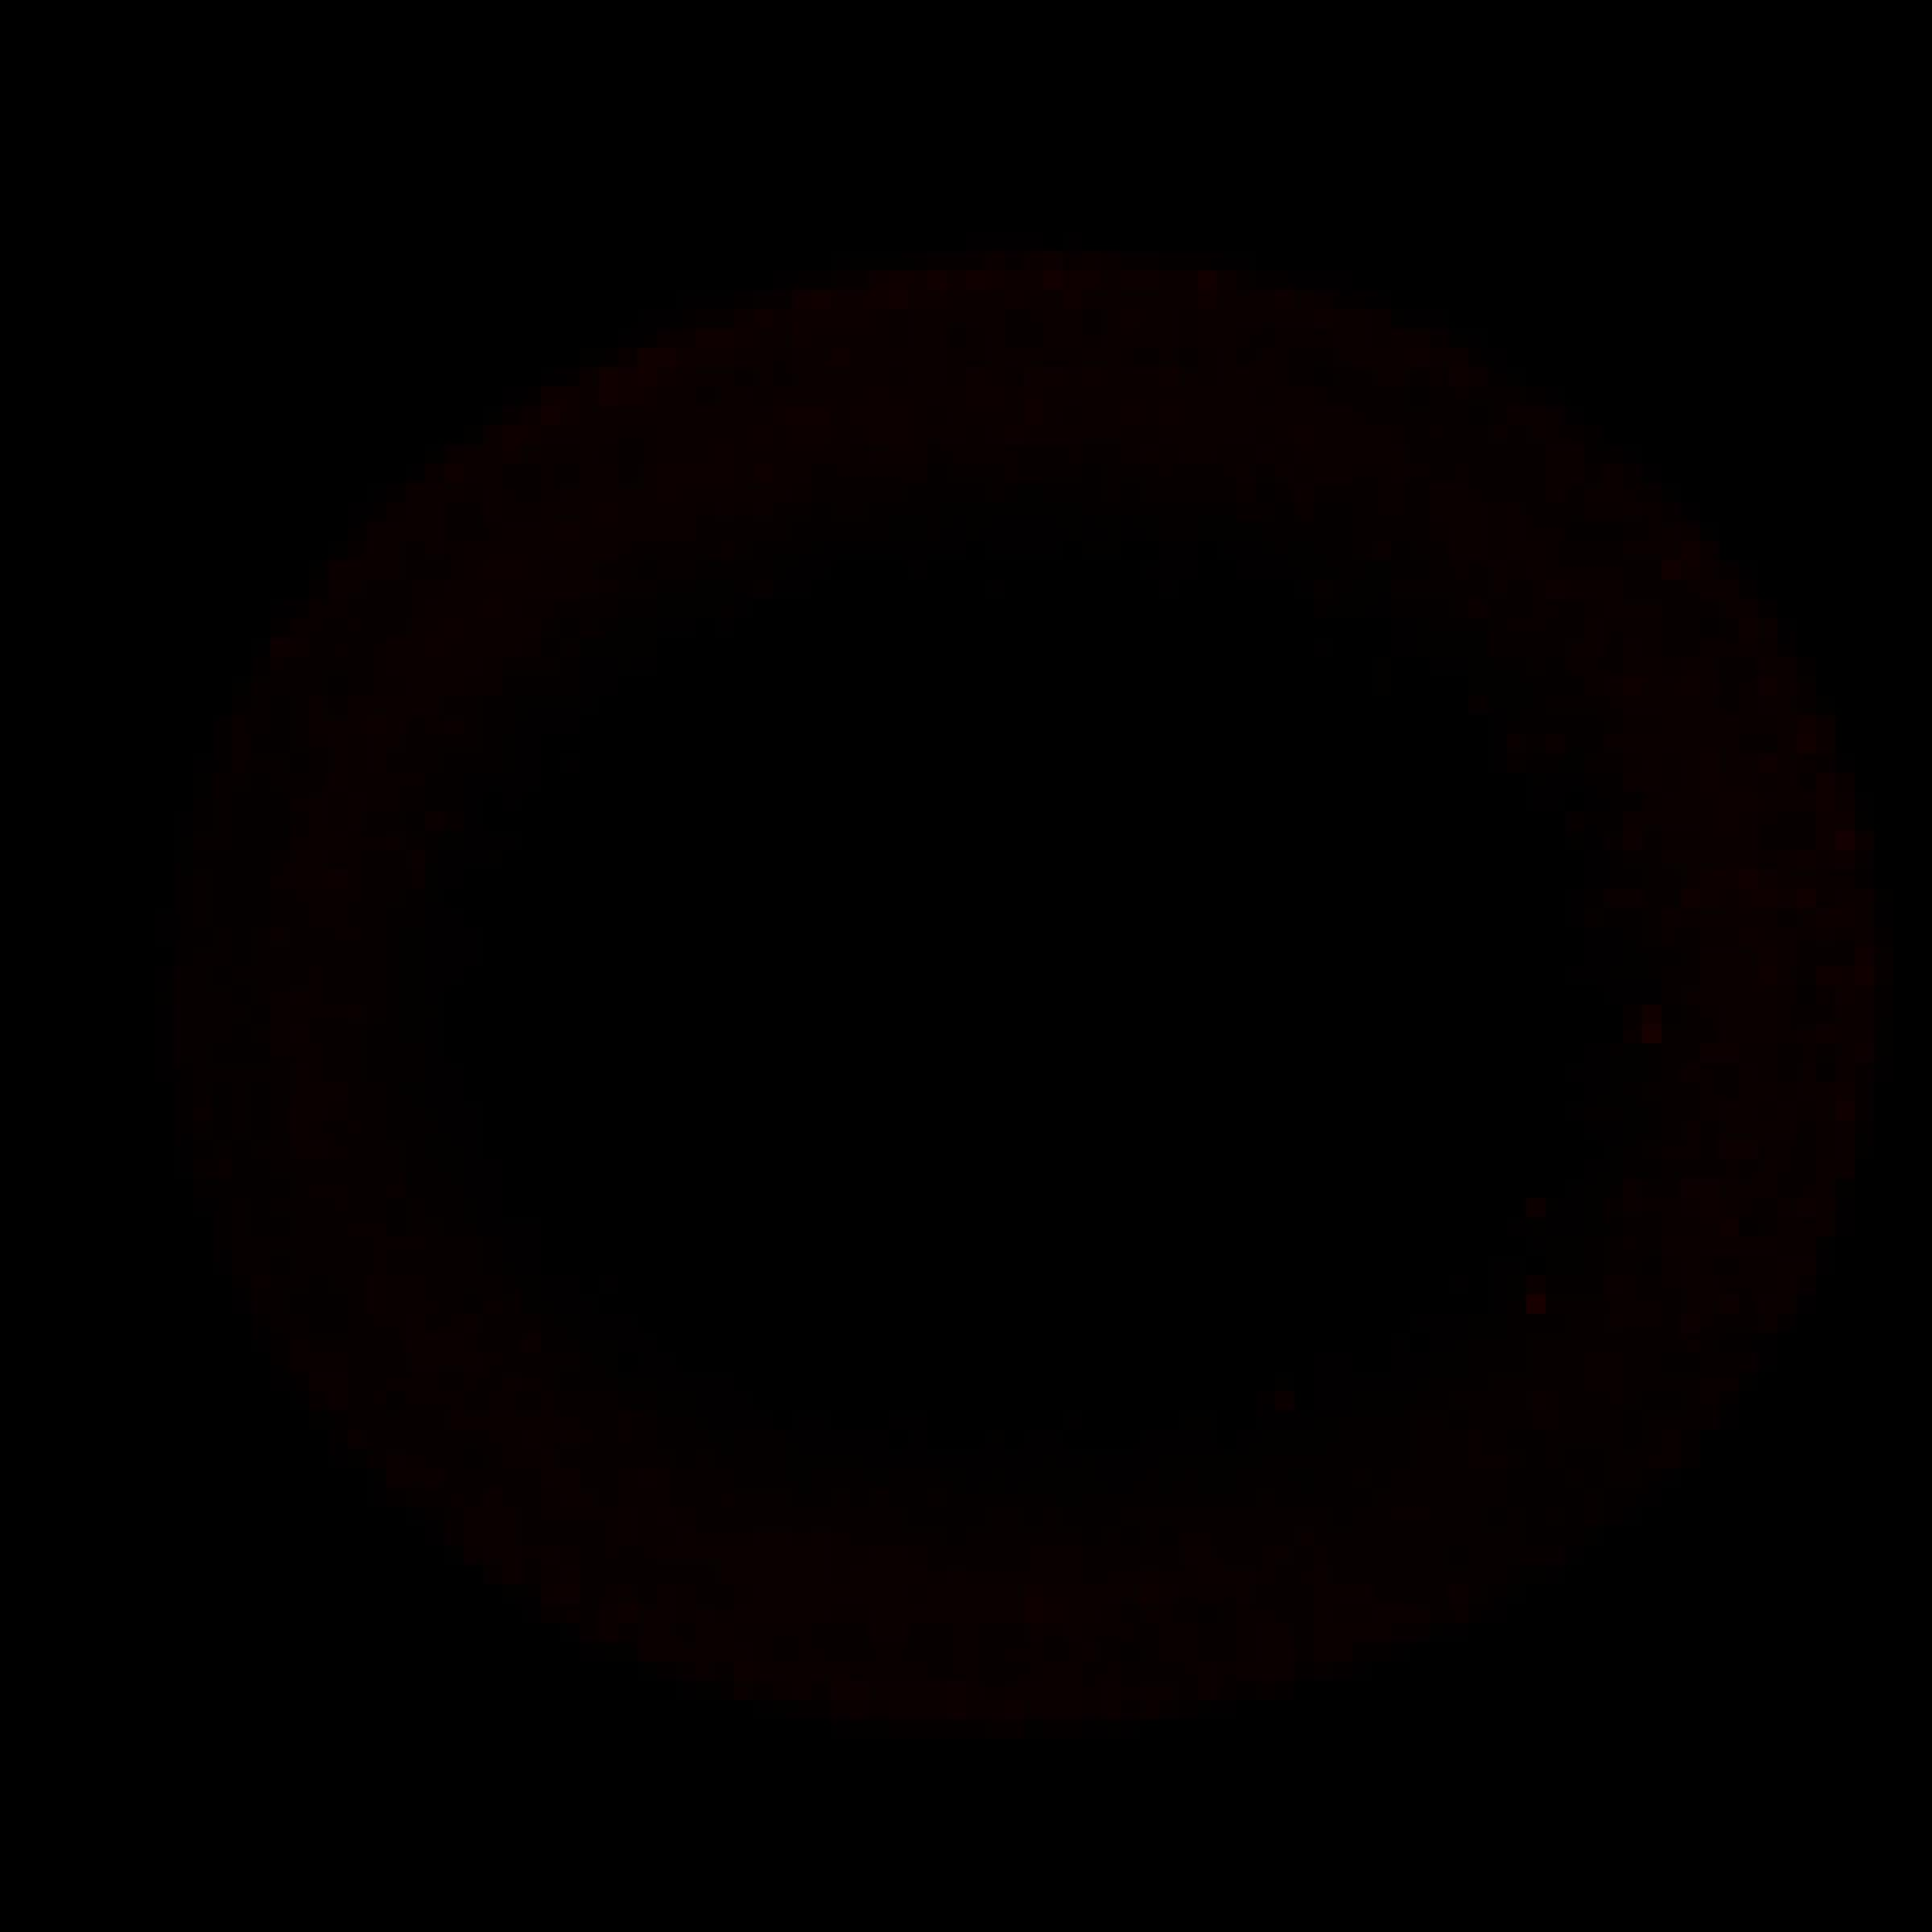
\includegraphics[width=0.15\textwidth]{dpERK_scat_1}};	
    	\node[right=0.1in of fig3](fig4) {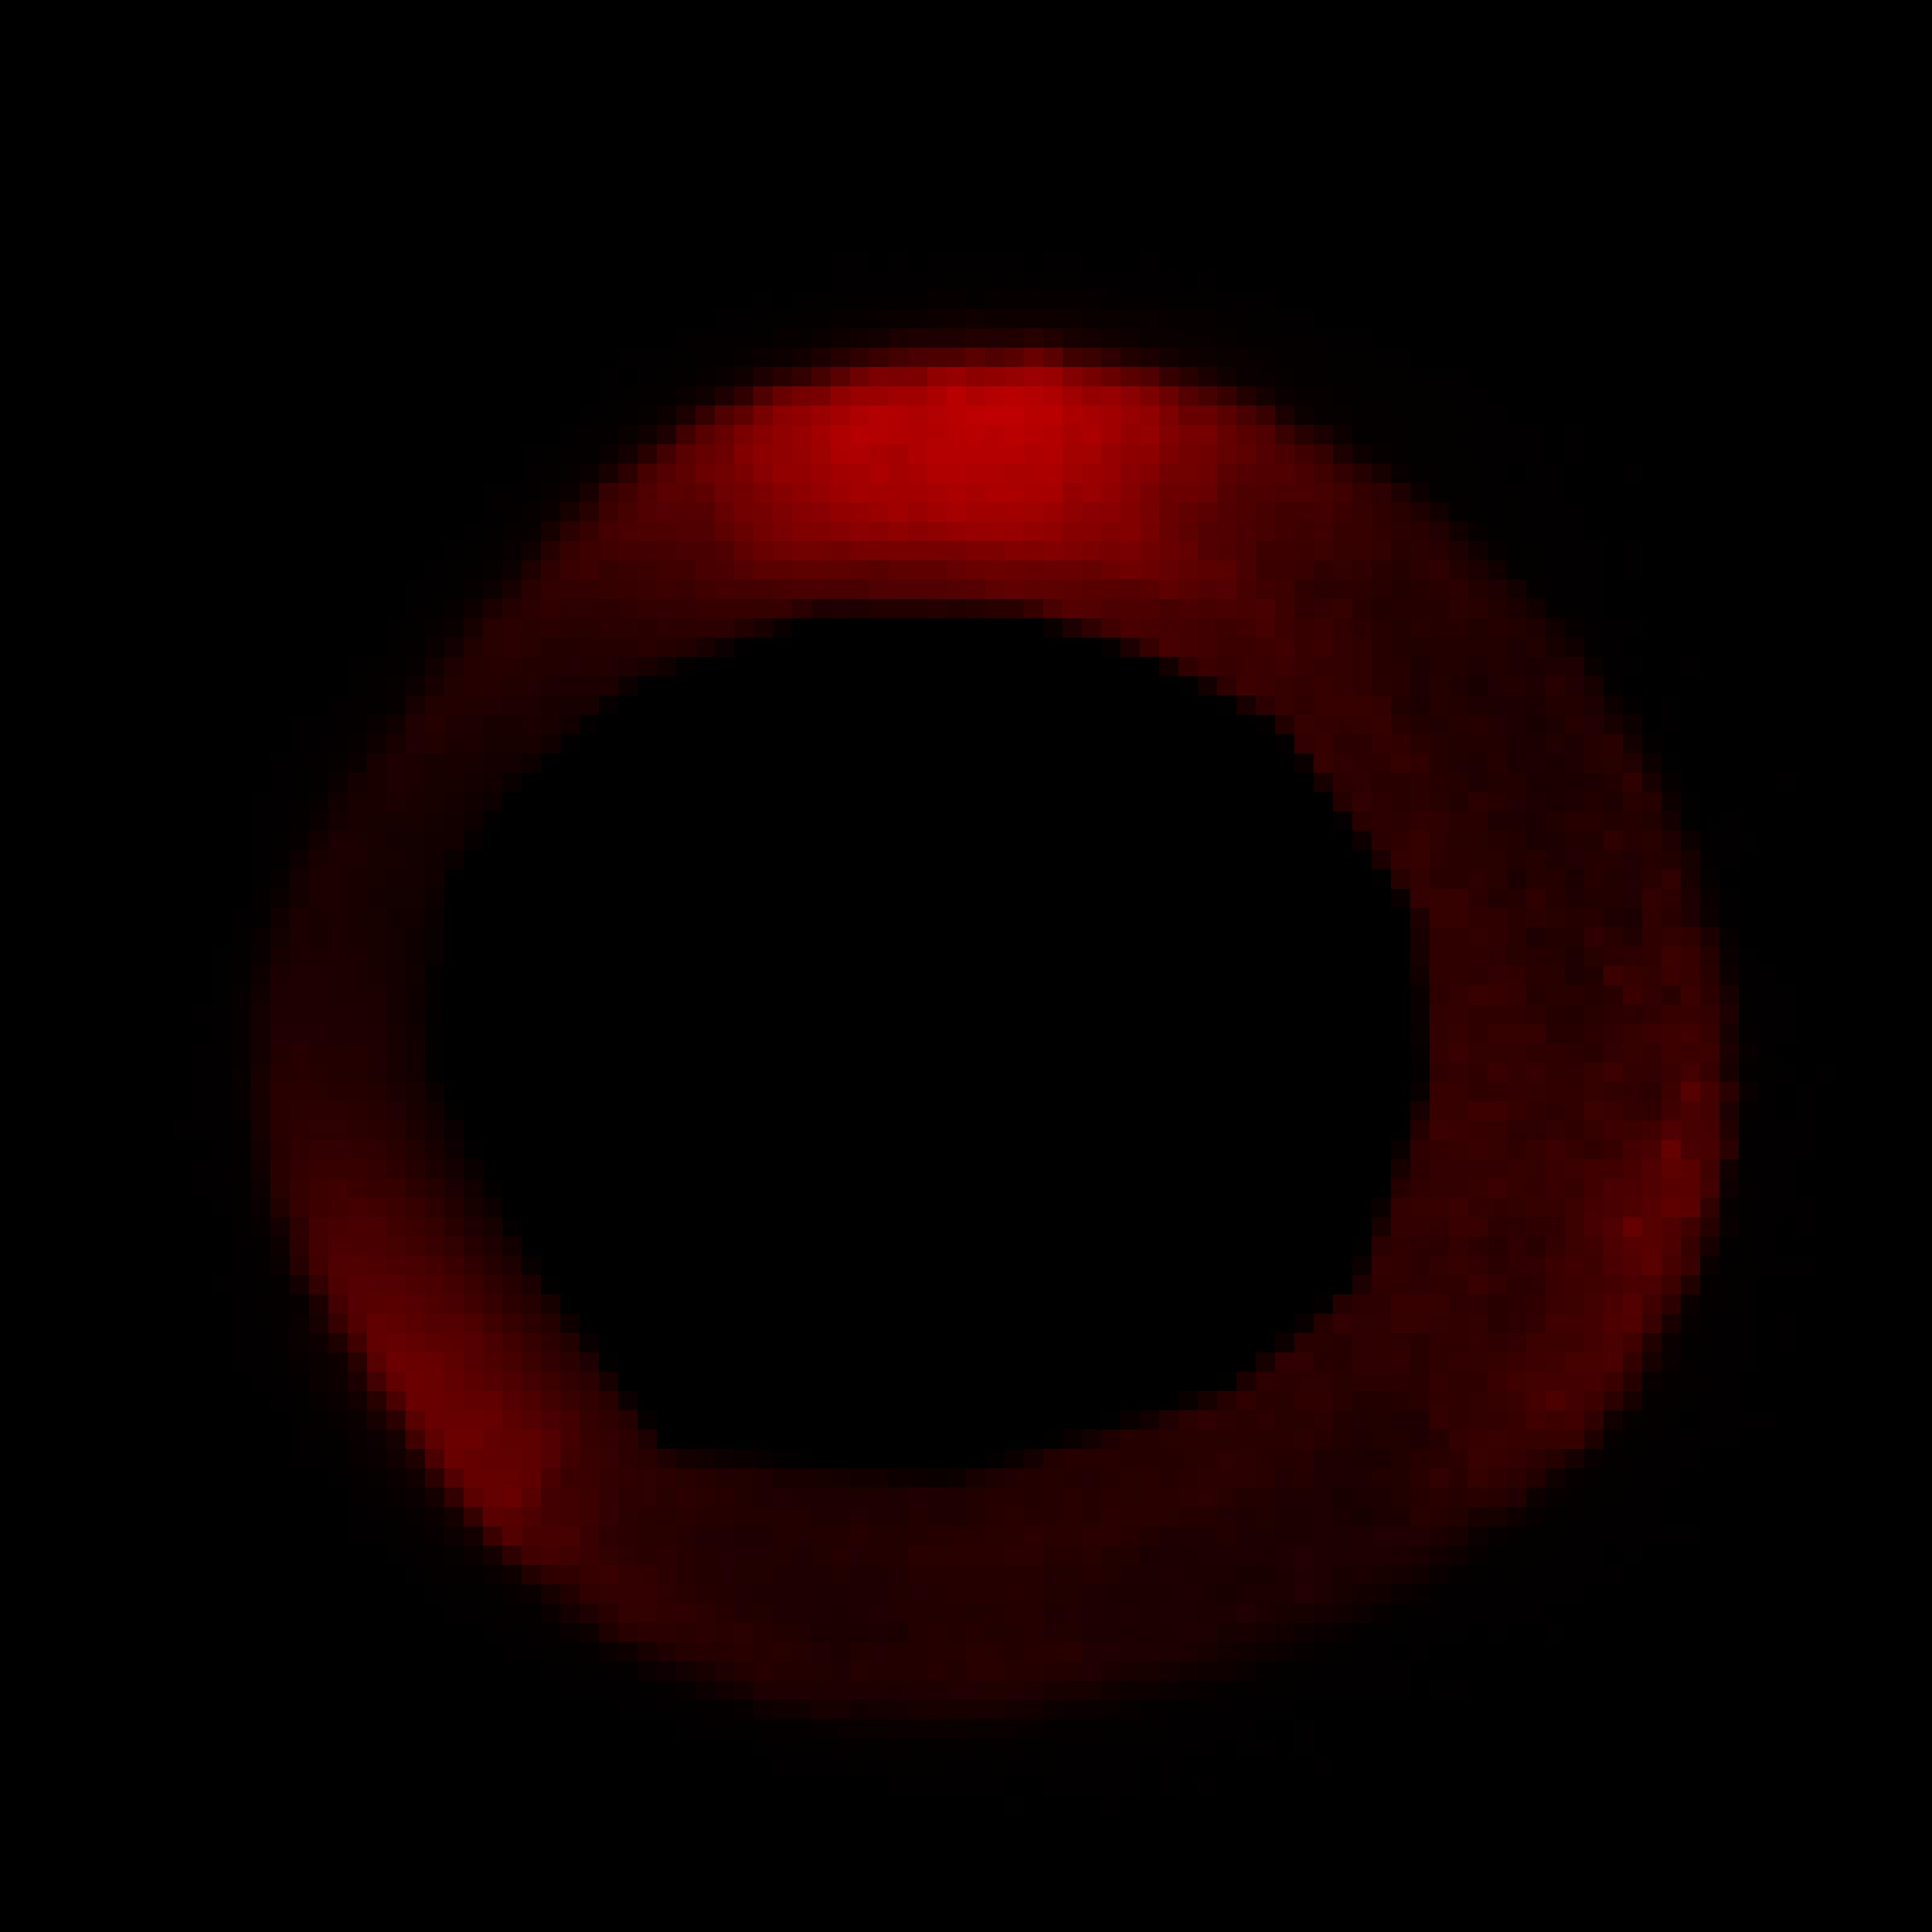
\includegraphics[width=0.15\textwidth]{dpERK_scat_4}};					
    	\node[right=0.1in of fig4](fig5) {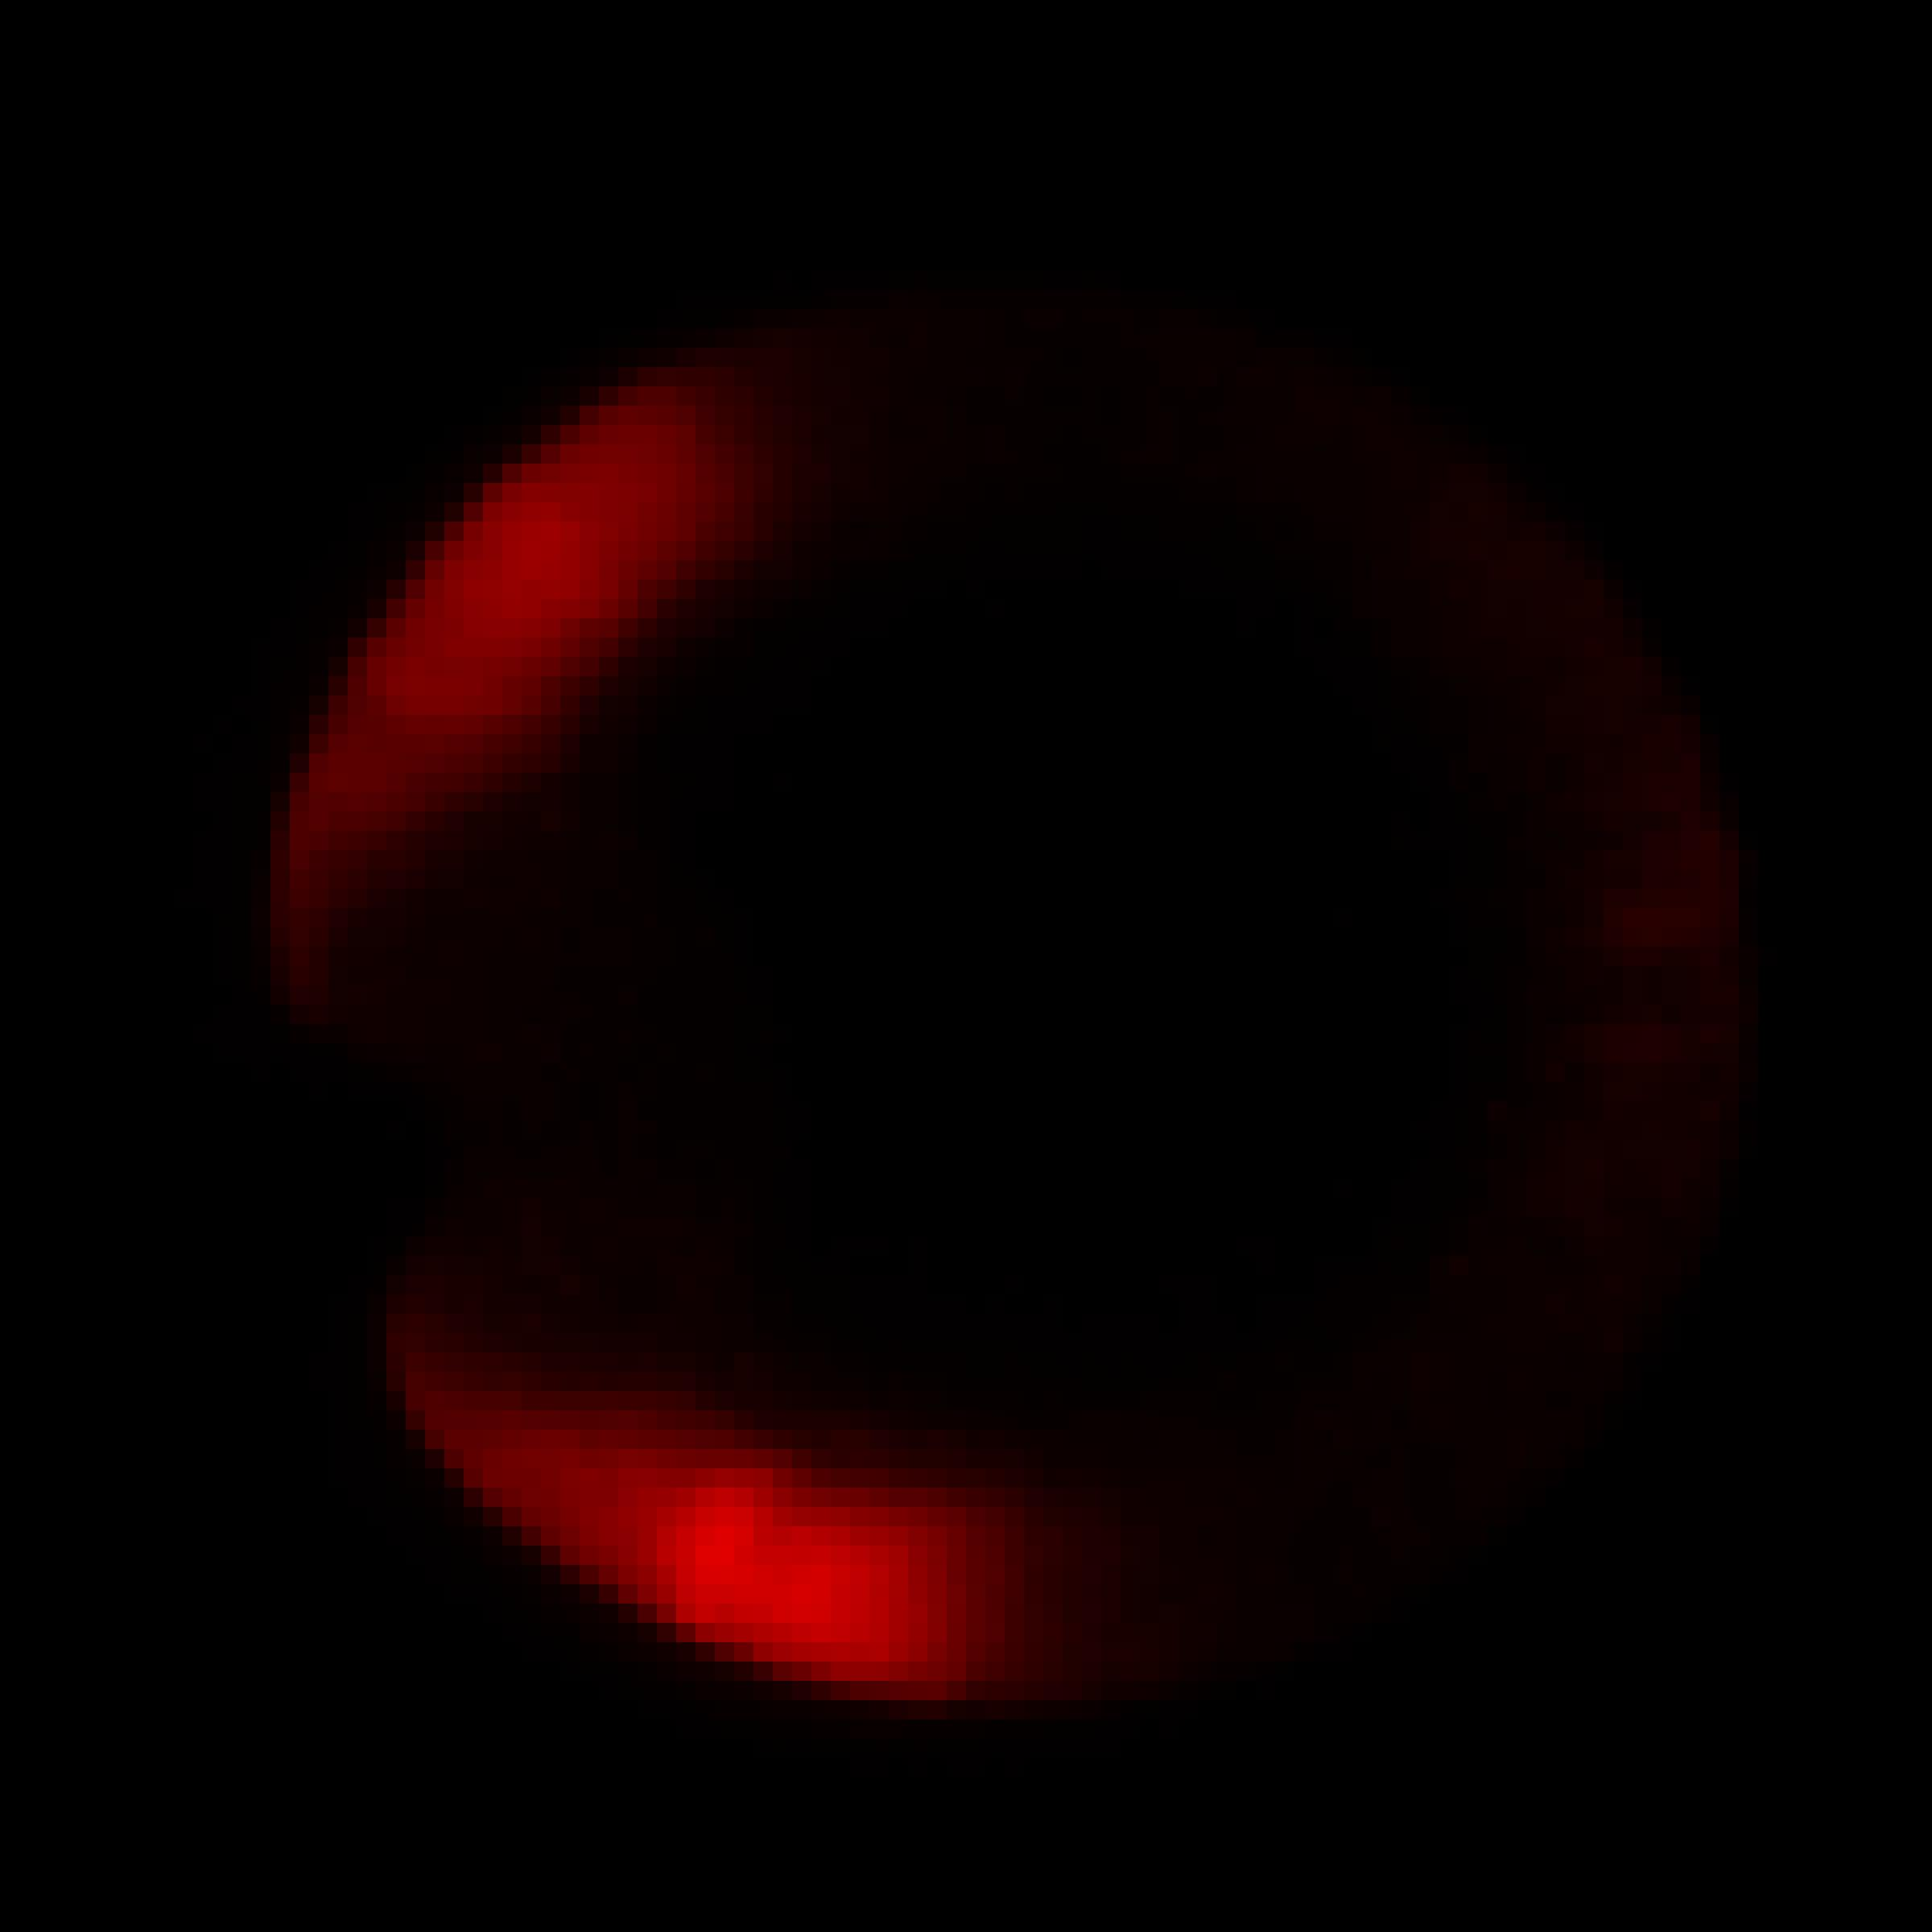
\includegraphics[width=0.15\textwidth]{dpERK_scat_5}};	    
    	\draw[->] (x1) -- (fig1.north);
    	\draw[->] (x2) -- (fig2.north);
    	\draw[->] (x3) -- (fig3.north);
    	\draw[->] (x4) -- (fig4.north);
    	\draw[->] (x5) -- (fig5.north);
    \end{tikzpicture}
    
\end{frame}

    
    

    